\documentclass[12pt,letterpaper]{article}

% ----------------- Packages -----------------
\usepackage[margin=1in]{geometry}
\usepackage{mathptmx}                 % Times-equivalent text + math
\usepackage[T1]{fontenc}
\usepackage{microtype}
\usepackage{graphicx}
\usepackage{caption}
\usepackage{subcaption}
\usepackage{booktabs}
\usepackage{multirow}
\usepackage{array}
\usepackage{amsmath, amssymb}
\usepackage{xcolor}
\usepackage{hyperref}
\usepackage{enumitem}
\usepackage{natbib}
\usepackage{float}
\usepackage{tabularx}
\usepackage{titlesec}

% ----------------- Layout -----------------
\setlength{\parskip}{3pt}
\setlength{\parindent}{0pt}
\linespread{1.0}    % single-spaced

\hypersetup{
  colorlinks=true,
  linkcolor=black,
  citecolor=blue!60!black,
  urlcolor=blue!60!black
}

\graphicspath{{figures/}}
\captionsetup[figure]{font=small, labelfont=bf, format=plain, justification=justified, skip=2pt}
\captionsetup[table]{font=small, labelfont=bf, format=plain, skip=2pt}

\titleformat{\section}{\bfseries\large}{\thesection.}{0.6em}{}
\titlespacing*{\section}{0pt}{8pt}{2pt}
\titleformat{\subsection}{\bfseries\normalsize}{\thesubsection}{0.6em}{}
\titlespacing*{\subsection}{0pt}{6pt}{1pt}

\pagestyle{empty}   % no headers, footers, or page numbers

\begin{document}

% ===================== TITLE PAGE =====================
\begin{titlepage}
\thispagestyle{empty}

\begin{figure}
    \centering
    \includegraphics[width=0.25\linewidth]{clipart544030.png}
\end{figure}
% Reserved space at the top for a logo (replace with \includegraphics
% or comment the \vspace if no logo is added)
\vspace*{3.5cm}

\begin{center}
{\Large\bfseries Analysis of U.S.\ Domestic Flight Delay Causes\\[4pt]
\normalsize An Inferential Study of Carrier, Seasonal, and Geographic\\[4pt]
Drivers of Flight Delays in 2024\par}

\vspace{18pt}
{\large DSE 501 Statistics for Data Analysts $|$ Spring C 2026 $|$ Team 8\par}

\vspace{60pt}

\begin{tabular*}{\textwidth}{@{\extracolsep{\fill}}ccc}
\textbf{James Czeranko}        & \textbf{\hspace{0.5cm}Ryan Garcia}          & \textbf{Yaksh Maulesh Pancholi}\\
Arizona State University       & \hspace{0.5cm}Arizona State University      & Arizona State University\\
\texttt{jczerank@asu.edu}      & \texttt{\hspace{0.3cm}rgarc203@asu.edu}     & \texttt{ypancho1@asu.edu}\\
\end{tabular*}

\vspace{18pt}
\begin{tabular}{c}
\textbf{Shaurya}\\
Arizona State University\\
\texttt{snola483@asu.edu}\\
\end{tabular}
\end{center}

\vfill
\end{titlepage}

% ===================== ABSTRACT (page 2) =====================
\noindent\textbf{Abstract.}
We analyze 15{,}046 carrier-airport-month records from the U.S.\ Department
of Transportation's Bureau of Transportation Statistics (BTS), covering
roughly 5.02~million arriving flights operated by 21 reporting carriers at
356 U.S.\ airports between January and August 2024. We apply one-way ANOVA,
Kruskal-Wallis, Tukey HSD, two-proportion z-tests, Pearson and Spearman
correlation, and ordinary least-squares (OLS) multiple regression to test
four pre-registered hypotheses concerning carrier identity, seasonality,
the relative impact of weather versus carrier-controllable causes, and the
relationship between airport flight volume and delay rate. We find strong,
highly significant evidence (all $p<10^{-10}$) that delay rates differ
across carriers and across months; that the share of delay minutes
attributable to carrier-controllable causes is more than five times the
share attributable to weather; and that larger airports experience higher
delay rates with a moderate, log-linear relationship. A nested-model
comparison shows that adding carrier identity to a baseline of seasonal
and volume effects more than doubles the explained variance ($R^2$:
$0.120 \!\rightarrow\! 0.256$), establishing carrier as the single most
important driver in our setting. A geographic extension on the four U.S.\
Census regions reveals a 2.5-percentage-point gap between the West
(lowest median delay rate) and the Midwest (highest).

\vspace{2pt}
\noindent\textbf{Keywords:} flight delay, ANOVA, Kruskal-Wallis, Tukey HSD,
two-proportion z-test, linear regression, BTS, on-time performance.

% ===================== SECTION 1 =====================
\section{Introduction and Problem Context}

\subsection{Background}
Flight delays are one of the most visible and costly inefficiencies of
modern air transportation. The Federal Aviation Administration estimates
that delays cost the U.S.\ economy tens of billions of dollars per year
through lost productivity, missed connections, additional fuel burn, and
crew rescheduling \citep{faa2024}. Beyond their direct economic impact,
delays propagate through the network: an aircraft that arrives late
becomes a delayed departure on its next leg, and a delay at a hub airport
can cascade across dozens of downstream destinations \citep{kafle2017}.
Understanding what drives delays, whether weather, air-traffic congestion,
carrier-controllable factors such as maintenance and crew scheduling, or
the propagation of late-arriving aircraft, is therefore central both
to airline operations and to public policy.

\subsection{Data Source and Collection}
The data are obtained from the U.S.\ Department of Transportation's
(DOT) Bureau of Transportation Statistics, which publishes the
\emph{Air Travel Consumer Report} on a monthly basis \citep{bts2024}.
Reporting carriers (those that account for at least one percent of
total domestic scheduled passenger revenue) are required to provide
on-time performance data for every domestic flight, broken down at the
carrier-airport-month level. For each delayed arrival, the carrier
reports the cause, classified into one of five mutually exclusive
categories defined by the DOT: \textbf{Air Carrier delay} (under the
carrier's control: maintenance, crew, baggage, fueling), \textbf{Extreme
Weather delay} (significant meteorological events such as tornadoes,
blizzards, hurricanes), \textbf{National Aviation System (NAS) delay}
(non-extreme weather, airport operations, heavy traffic volume,
air-traffic-control limitations), \textbf{Late-Arriving Aircraft delay}
(a previous flight using the same airframe arrived late), and
\textbf{Security delay} (re-screening, evacuations, breaches).

\subsection{Dataset Characteristics}
After dropping 14 records (0.09\%) with missing values, our analytical
dataset contains $n = 15{,}046$ carrier-airport-month records spanning
January through August 2024, covering 21 carriers and 356 airports. Each
record contains 21 variables, including total arriving flights
(\texttt{arr\_flights}), flights delayed by 15 minutes or more
(\texttt{arr\_del15}), total delay minutes across all delayed flights
(\texttt{arr\_delay}), and both the count and the total minutes of each
of the five delay causes. In aggregate the dataset captures
\textbf{5{,}022{,}488} flights, of which \textbf{1{,}129{,}387}
(22.49\%) were delayed by 15 minutes or more.

\subsection{Hypotheses of Interest}
We pre-registered four hypotheses in our project proposal. Throughout,
we follow the standard Neyman-Pearson framework: $H_0$ is the null
hypothesis of no effect, $H_1$ the alternative, and we fix the
significance level at $\alpha = 0.05$.
\begin{itemize}[leftmargin=2.0em, itemsep=2pt, topsep=2pt]
  \item \textbf{H1 (Carrier effect):} $H_0$: the mean delay rate does
  not differ across the 21 carriers; $H_1$: at least one carrier differs.
  \item \textbf{H2 (Seasonality):} $H_0$: the mean delay rate is constant
  across the eight months; $H_1$: it varies by month.
  \item \textbf{H3 (Weather vs.\ Carrier):} $H_0$: the share of total
  delay minutes attributable to weather equals the share attributable to
  carrier-controllable causes; $H_1$: the two shares differ.
  \item \textbf{H4 (Volume-vs-rate correlation):} $H_0$: airport flight
  volume and delay rate are linearly uncorrelated; $H_1$: a positive
  correlation exists.
\end{itemize}

\subsection{Importance of the Solution and Relevant Literature}
Quantifying the relative contribution of each cause has direct
implications for resource allocation. If carrier-controllable factors
dominate, regulatory and contractual incentives to invest in
maintenance, crew scheduling and turn-time discipline are warranted; if
NAS or weather factors dominate, the lever shifts toward infrastructure
investment and air-traffic-control modernization.

The statistical analysis of flight delays has a substantial literature.
\citet{tu2008} model the long-term and seasonal structure of departure
delay distributions; \citet{rebollo2014} use random forests to predict
network-wide air-traffic delays and identify hub centrality as a leading
predictor; \citet{mukherjee2014} formalize the trade-off between ground
delay programs and airborne delay under capacity uncertainty;
\citet{abdelghany2004} report clear weekly and monthly periodicities in
arrival delays; and \citet{kafle2017} develop a propagation model that
explicitly tracks late-arriving-aircraft cascades, finding that roughly
one-third of delays in any given period stem from earlier delays in the
same airframe's itinerary. Our work is a descriptive and inferential
study in this tradition: we do not predict individual flights, but
instead apply classical hypothesis tests to isolate the
causal-attribution structure of delays in the most recent publicly
available BTS panel.

% ===================== SECTION 2 =====================
\section{Exploratory Data Analysis}

\subsection{Derived Metrics and Preprocessing}
Two derived metrics anchor our analysis. The \emph{delay rate} is
$\text{delay\_rate}_i = \text{arr\_del15}_i / \text{arr\_flights}_i$,
i.e.\ the fraction of arrivals delayed by 15 or more minutes. The
\emph{average delay duration} is
$\text{avg\_delay\_min}_i = \text{arr\_delay}_i / \text{arr\_del15}_i$
when $\text{arr\_del15}_i > 0$, and zero otherwise. The first captures
\emph{frequency} (how often flights are late) and the second captures
\emph{severity} (how long delays last). Normalizing by the number of
arrivals removes scale effects so a small regional carrier and a
megahub can be compared on the same footing. We also remove 14 records
with missing values, leaving $n=15{,}046$.

\subsection{Delay-Cause Composition}
Figure~\ref{fig:cause} shows the marginal breakdown of delays by cause
across the entire dataset, and Table~\ref{tab:cause} reports the same
numbers in a compact form.

\begin{figure}[!htbp]
  \centering
  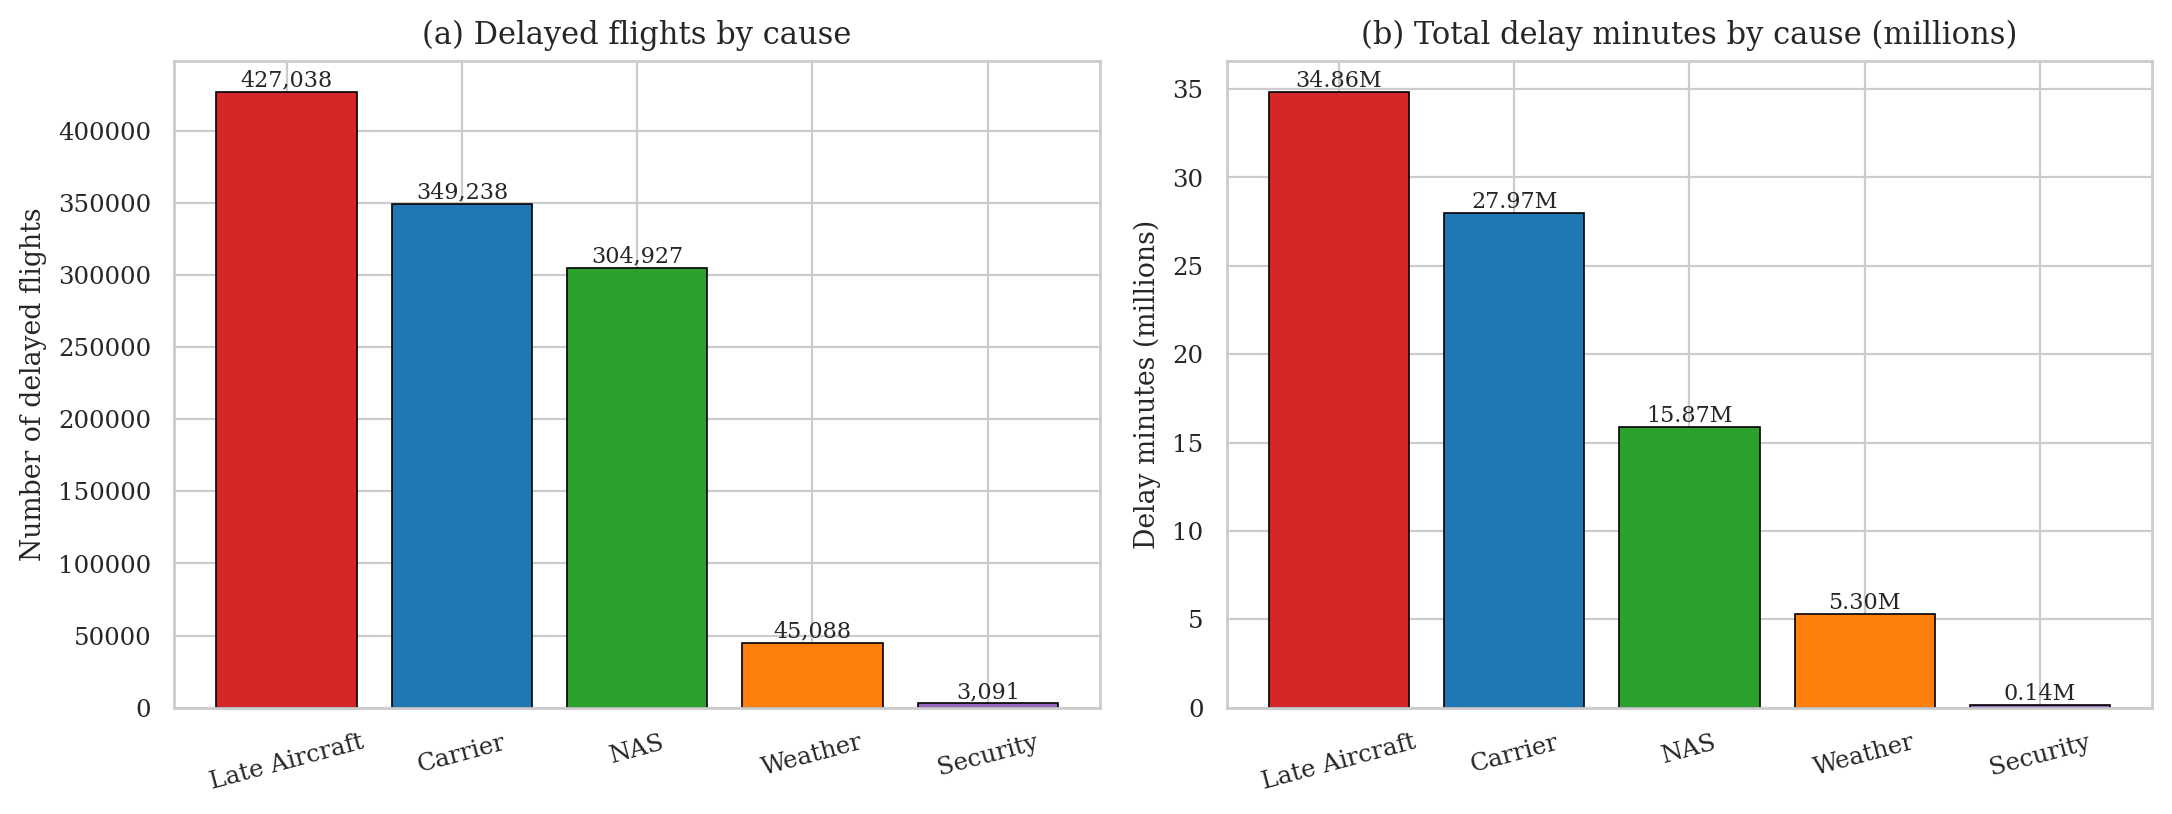
\includegraphics[width=\linewidth]{fig_cause_breakdown}
  \caption{Marginal breakdown of delayed flights and total delay minutes
  by DOT cause category, January--August 2024. Late-arriving aircraft
  and carrier-controllable factors together account for 68.7\% of all
  delayed flights and 74.7\% of all delay minutes.}
  \label{fig:cause}
\end{figure}

\begin{table}[H]
\centering
\caption{Delay cause breakdown across all carrier--airport--month
records, January--August 2024. Average minutes per flight divides total
attributed minutes by all 5{,}022{,}488 arrivals.}
\label{tab:cause}
\small
\begin{tabular}{lrrrr}
\toprule
\textbf{Delay cause} & \textbf{Delayed flights} & \textbf{\% of delays} &
\textbf{Total minutes} & \textbf{Avg.\ min/flight}\\
\midrule
Late Aircraft     & 427{,}038 & 37.81\% & 34{,}864{,}194 & 6.94 \\
Carrier           & 349{,}238 & 30.92\% & 27{,}974{,}948 & 5.57 \\
NAS               & 304{,}927 & 27.00\% & 15{,}868{,}049 & 3.16 \\
Weather           &  45{,}088 &  3.99\% &  5{,}298{,}959 & 1.06 \\
Security          &   3{,}091 &  0.27\% &     139{,}693  & 0.03 \\
\midrule
\textbf{Total}    & \textbf{1{,}129{,}382} & \textbf{100.00\%} &
\textbf{84{,}145{,}843} & \textbf{16.76} \\
\bottomrule
\end{tabular}
\end{table}

Two patterns dominate. Late-arriving aircraft is the largest single
cause both by count (37.8\%) and by minutes (41.4\%), consistent with
the propagation hypothesis of \citet{kafle2017}. Carrier-controllable
causes contribute another 30.9\% of delays and 33.2\% of minutes,
nearly five times the share attributable to weather; security is
negligible.

\subsection{Variation across Carriers and Months}
Figure~\ref{fig:carrier} plots the delay-rate distribution for each of
the 21 carriers, sorted by median. The visual evidence of
between-carrier variation is substantial: the median rate for the best
carrier (PT, Piedmont) sits below 0.13, while the worst (AA, American)
is around 0.30, a more than two-fold difference. The interquartile
ranges are also wider for high-mean carriers, suggesting carriers with
high overall delay rates also have higher \emph{within-carrier}
variability across airports and months.

\begin{figure}[!htbp]
  \centering
  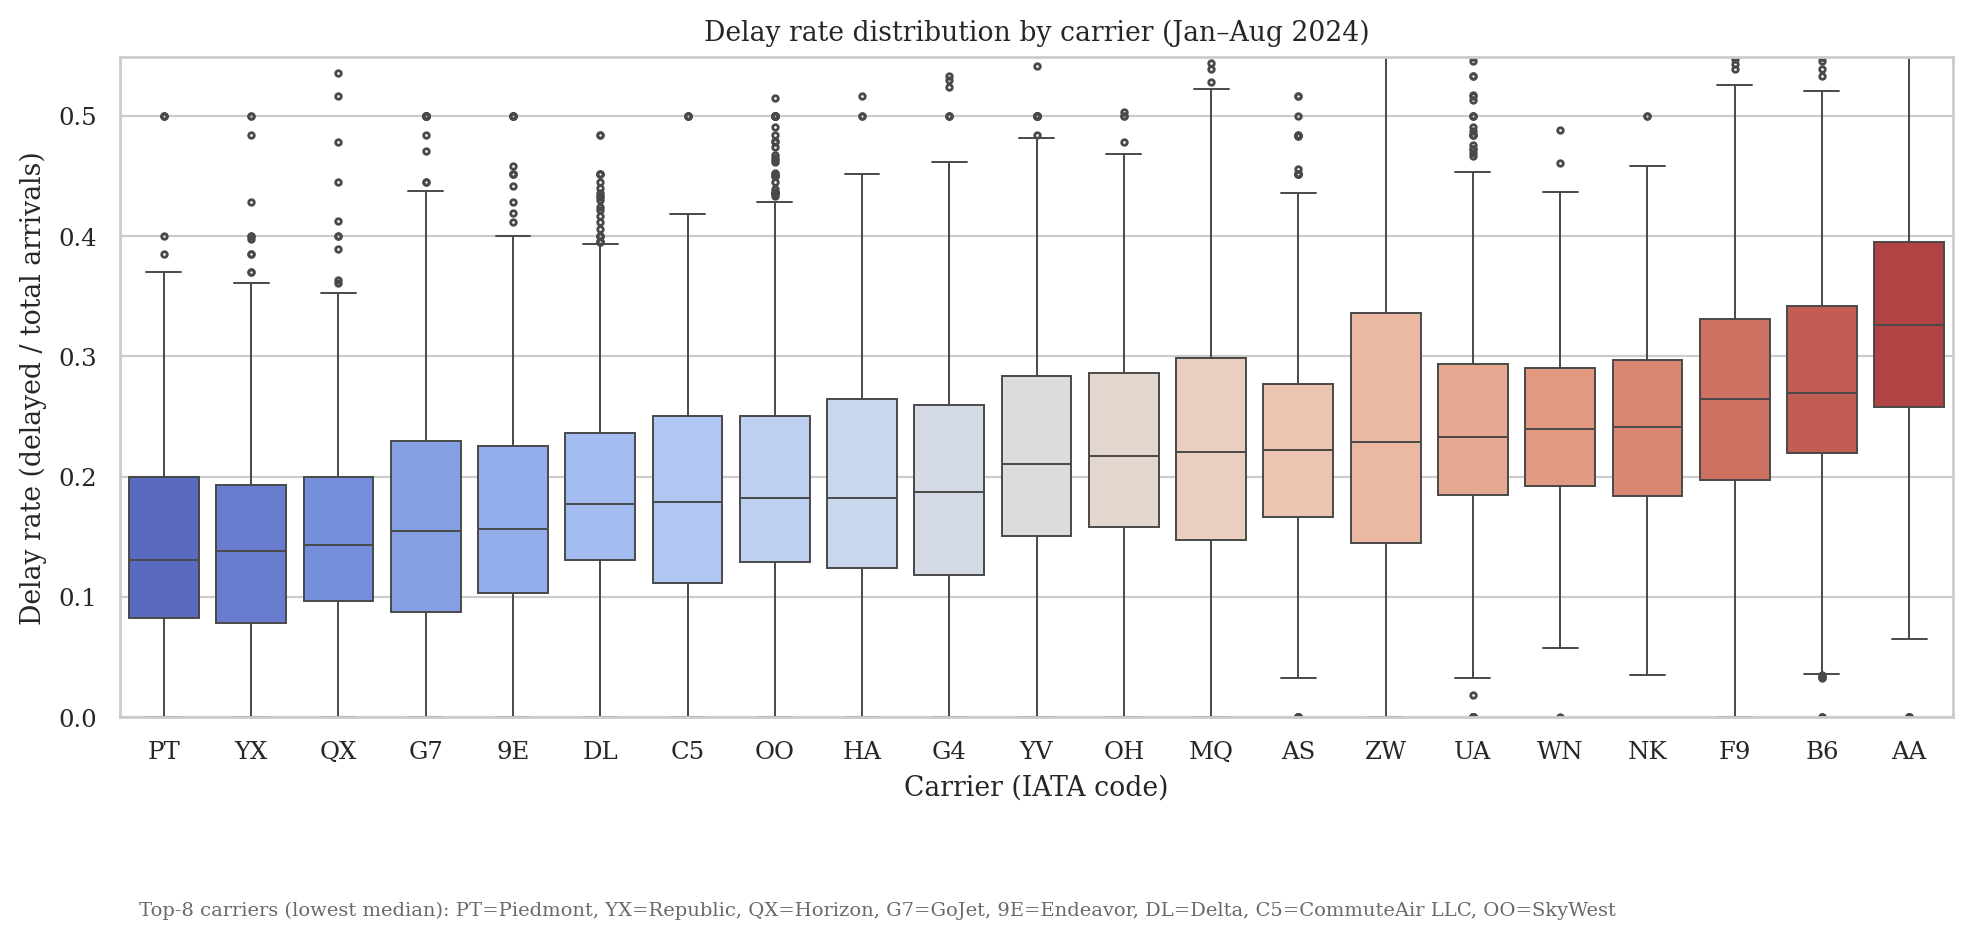
\includegraphics[width=0.9\linewidth]{fig_carrier_delay_rate}
  \caption{Delay-rate distributions for all 21 reporting carriers,
  sorted by median (top axis truncated at the 99th percentile).}
  \label{fig:carrier}
\end{figure}

Figure~\ref{fig:monthly} pairs the monthly trend with its compositional
breakdown. Mean delay rate falls from January through February (the
post-holiday lull), rises sharply through spring and summer, peaks in
July ($\approx 0.28$), and recedes in August. Compositional shifts are
informative: weather's share of total delay minutes is highest in
January (10.9\%) and lowest in July (4.6\%), while carrier and
late-aircraft together rise from 72\% in January to 79\% in July. This is
exactly what one would expect operationally, since summer thunderstorms
produce frequent but moderate NAS delays rather than the rare
extreme-weather events that dominate winter.

\begin{figure}[!htbp]
  \centering
  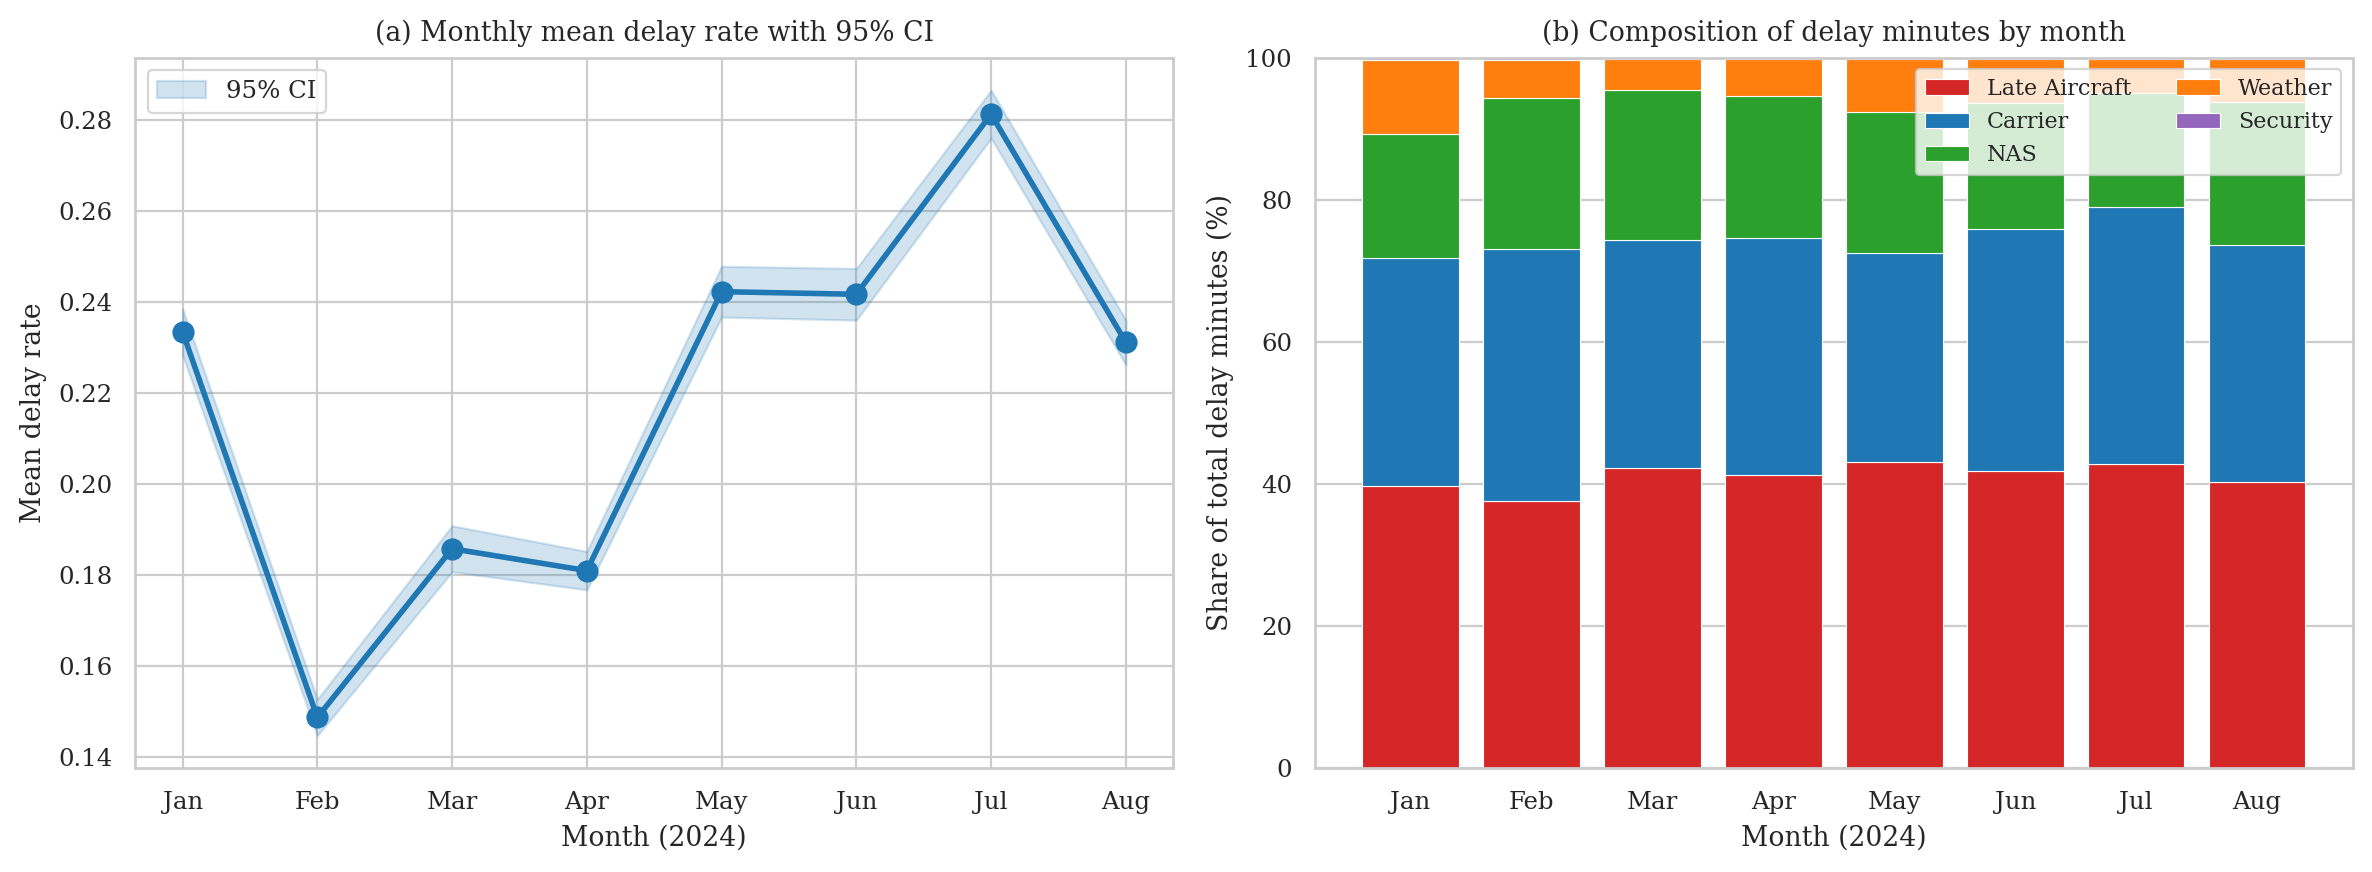
\includegraphics[width=\linewidth]{fig_monthly_trend}
  \caption{Monthly trends. (a) Mean delay rate by month with 95\%
  confidence intervals; February is the calmest month and July the
  worst. (b) Composition of total delay minutes; carrier and
  late-aircraft shares rise during the summer travel peak.}
  \label{fig:monthly}
\end{figure}

The carrier-by-month interaction is read from Figure~\ref{fig:heatmap}.
Highest-mean carriers (bottom rows) are noticeably warmer across nearly
every month, indicating that the carrier ranking is broadly stable
through 2024.

\begin{figure}[!htbp]
  \centering
  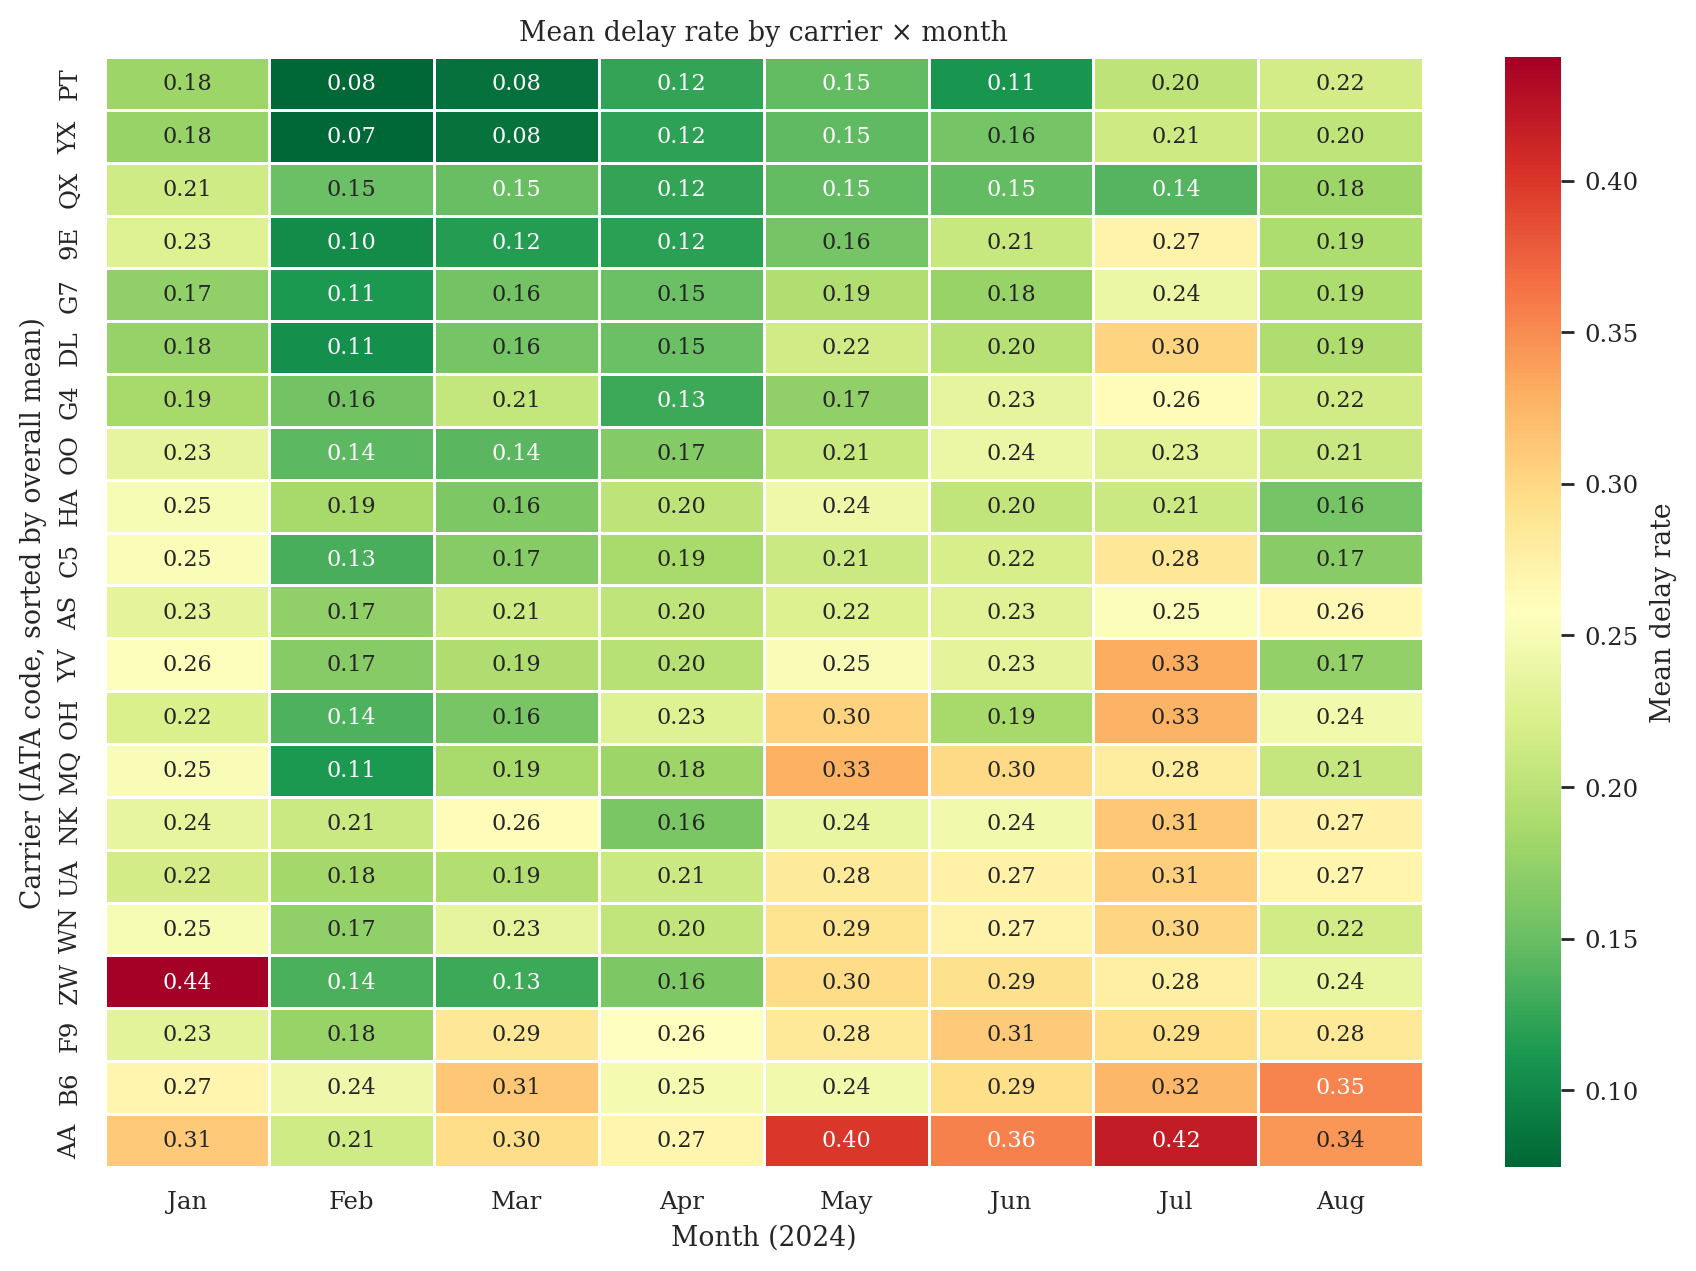
\includegraphics[width=0.74\linewidth]{fig_heatmap_carrier_month}
  \caption{Mean delay rate by carrier and month, rows sorted by overall
  mean. Isolated anomalies remain (e.g.\ ZW spikes to 0.44 in January).}
  \label{fig:heatmap}
\end{figure}

\subsection{Airport Volume vs.\ Delay Rate, and Initial Data-Quality Issues}
Figure~\ref{fig:volume} plots each of the 350 airports with at least 100
flights as a single point. The visual relationship is positive but
noisy: among the megahubs (DFW, LAS, CLT, ORD, DEN, LAX, PHX, ATL),
only ATL falls below the median delay rate, and DFW is the
worst-performing megahub.

\begin{figure}[!htbp]
  \centering
  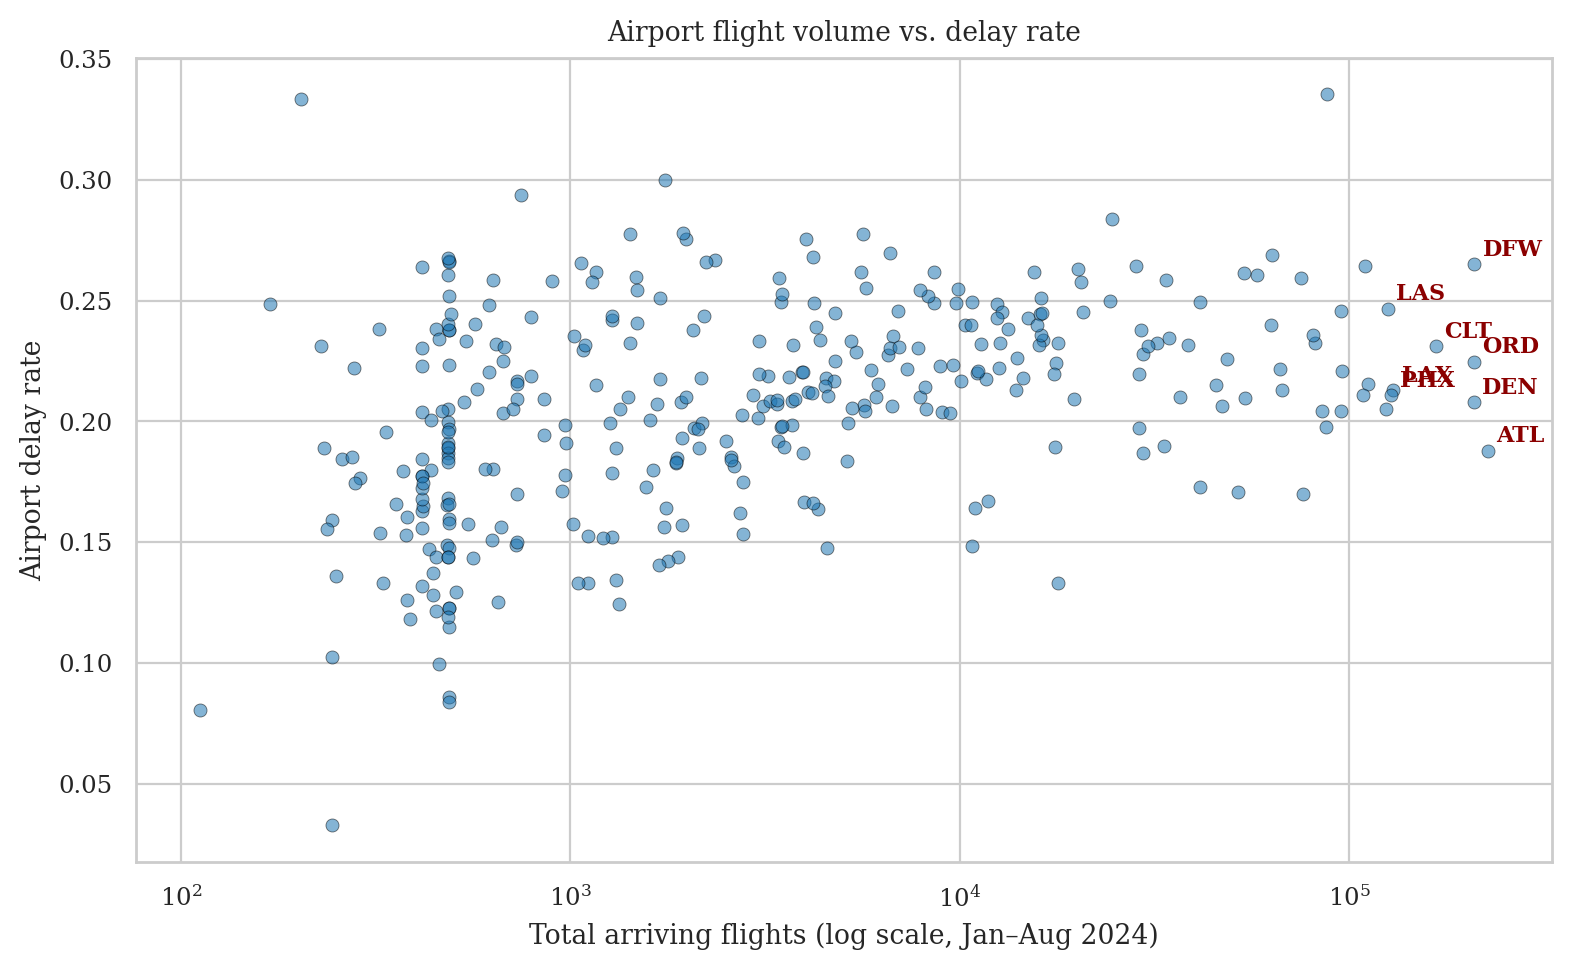
\includegraphics[width=0.7\linewidth]{fig_volume_vs_rate}
  \caption{Airport-level scatter of total arriving flights (log scale)
  vs.\ delay rate, January--August 2024.}
  \label{fig:volume}
\end{figure}

Two issues surfaced in this exploratory phase. First, normality is
clearly violated: a Shapiro-Wilk test on a 5{,}000-record random sample
gives $W = 0.938$, $p < 10^{-10}$, and visual inspection shows
pronounced right skew driven by long upper tails of small carriers in
poor weather. Second, Levene's test rejects equal variances at
$W = 19.75$, $p < 10^{-10}$. Both diagnostics imply the parametric
ANOVA assumptions for H1 and H2 may not hold; we therefore complement
every ANOVA in Section~\ref{sec:inferential} with a non-parametric
Kruskal-Wallis test, and treat the latter as the primary inferential
instrument.

% ===================== SECTION 3 =====================
\section{Inferential Data Analysis}
\label{sec:inferential}

We now formally test the four hypotheses at $\alpha = 0.05$. For each
hypothesis we (a) state the test, (b) check its assumptions, (c) report
the test statistic, (d) where appropriate follow up with post-hoc
pairwise comparisons, and (e) give the substantive interpretation.
Implementation uses \texttt{scipy.stats} \citep{virtanen2020}.

\subsection{H1: Carrier Effect on Delay Rate}
\textbf{Test.} One-way ANOVA on \texttt{delay\_rate} grouped by
\texttt{carrier} ($k = 21$ groups, $N = 15{,}046$).

\textbf{Assumption checks.} Shapiro-Wilk on a random sample of 5{,}000
records yields $W = 0.938$, $p < 10^{-10}$ (normality rejected).
Levene's median-centered test yields $W = 19.75$, $p < 10^{-10}$ (equal
variances rejected). Both ANOVA assumptions are violated, motivating
the non-parametric backup.

\textbf{Test statistics.} Despite the assumption violations the ANOVA
$F$-statistic is highly significant: $F(20, 15{,}025) = 124.48$,
$p < 10^{-10}$. The non-parametric Kruskal-Wallis test gives
$H = 2{,}663.83$, $p < 10^{-10}$. Both reject $H_0$. The eta-squared
effect size is
$\eta^2 = \mathrm{SS}_{\mathrm{between}}/\mathrm{SS}_{\mathrm{total}} = 0.142$,
i.e.\ carrier identity alone explains roughly 14.2\% of the variance in
the record-level delay rate, a large effect by the conventions of
\citet{montgomery2017}.

\textbf{Post-hoc.} Tukey HSD restricted to the eight carriers with the
largest sample size yields significant differences in 21 of 28 pairs
(75\%). The two large carriers AA and B6 differ from every other top-8
carrier; the regional pair OO and YV are statistically
indistinguishable. \textbf{Decision: reject $H_0$.}

\subsection{H2: Seasonal Variation}
\textbf{Test.} One-way ANOVA on \texttt{delay\_rate} grouped by
\texttt{month}. Levene's test gives $W = 35.04$, $p < 10^{-10}$, again
rejecting equal variances. ANOVA: $F(7, 15{,}038) = 276.76$,
$p < 10^{-10}$. Kruskal-Wallis: $H = 2{,}174.47$, $p < 10^{-10}$.
Eta-squared $\eta^2 = 0.114$.

\textbf{Post-hoc Tukey HSD.} Of the $\binom{8}{2} = 28$ month pairs, 22
(78.6\%) differ significantly. Figure~\ref{fig:tukey} visualizes the
full pairwise p-value matrix.

\begin{figure}[!htbp]
  \centering
  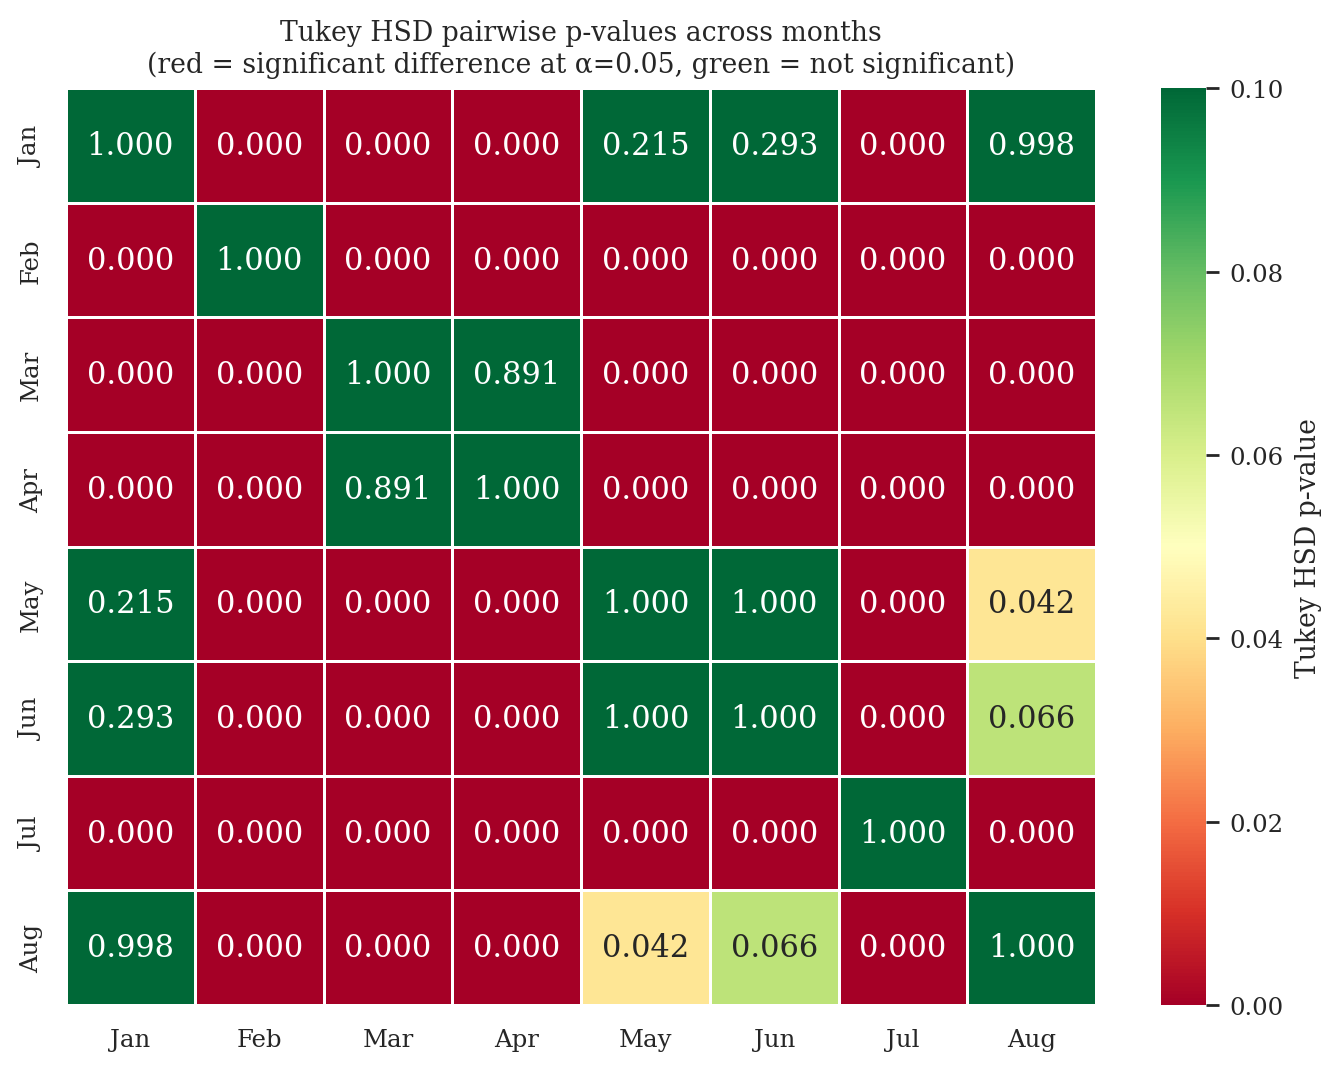
\includegraphics[width=0.62\linewidth]{fig_h2_tukey_heatmap}
  \caption{Tukey HSD pairwise p-values across months. Red cells are
  pairs that differ significantly at $\alpha=0.05$. The only
  non-significant pairs are Mar--Apr ($p=0.891$), Jan--Aug ($p=0.998$),
  May--Jun ($p=1.000$), Jan--May ($p=0.215$), and Jan--Jun ($p=0.293$).}
  \label{fig:tukey}
\end{figure}

\textbf{Decision: reject $H_0$.} The post-hoc structure further reveals
that the eight months partition into roughly three regimes: a low-delay
band (February--April), a transition (January, May, June, August), and
a peak (July).

\subsection{H3: Weather vs.\ Carrier as Delay Drivers}
\textbf{Test.} Two-proportion z-test on the share of total delay minutes
attributable to weather versus the share attributable to
carrier-controllable causes. Total delay minutes across all five causes
is $T = 84{,}145{,}843$. The weather and carrier components are
$W = 5{,}298{,}959$ and $C = 27{,}974{,}948$ respectively. Treating
each as a count out of $T$, we test $H_0: p_W = p_C$ versus
$H_1: p_W \neq p_C$. The pooled-variance z statistic is
\begin{equation}
  z \;=\; \frac{\hat p_W - \hat p_C}
              {\sqrt{\hat p_{\mathrm{pool}}(1-\hat p_{\mathrm{pool}})
                     \left(\tfrac{1}{T} + \tfrac{1}{T}\right)}}.
\end{equation}
We obtain $\hat p_W = 0.0630$, $\hat p_C = 0.3325$, difference
$\hat p_W - \hat p_C = -0.2695$ with a 95\% Wald confidence interval of
$[-0.2696, -0.2694]$, $z = -4{,}388.84$, $p < 10^{-10}$. As a sanity
check we re-ran the test on counts of delayed flights:
$\hat p_W = 0.0399$, $\hat p_C = 0.3092$, $z = -533.12$, $p < 10^{-10}$,
showing the same direction and effect-size ranking.

\begin{figure}[!htbp]
  \centering
  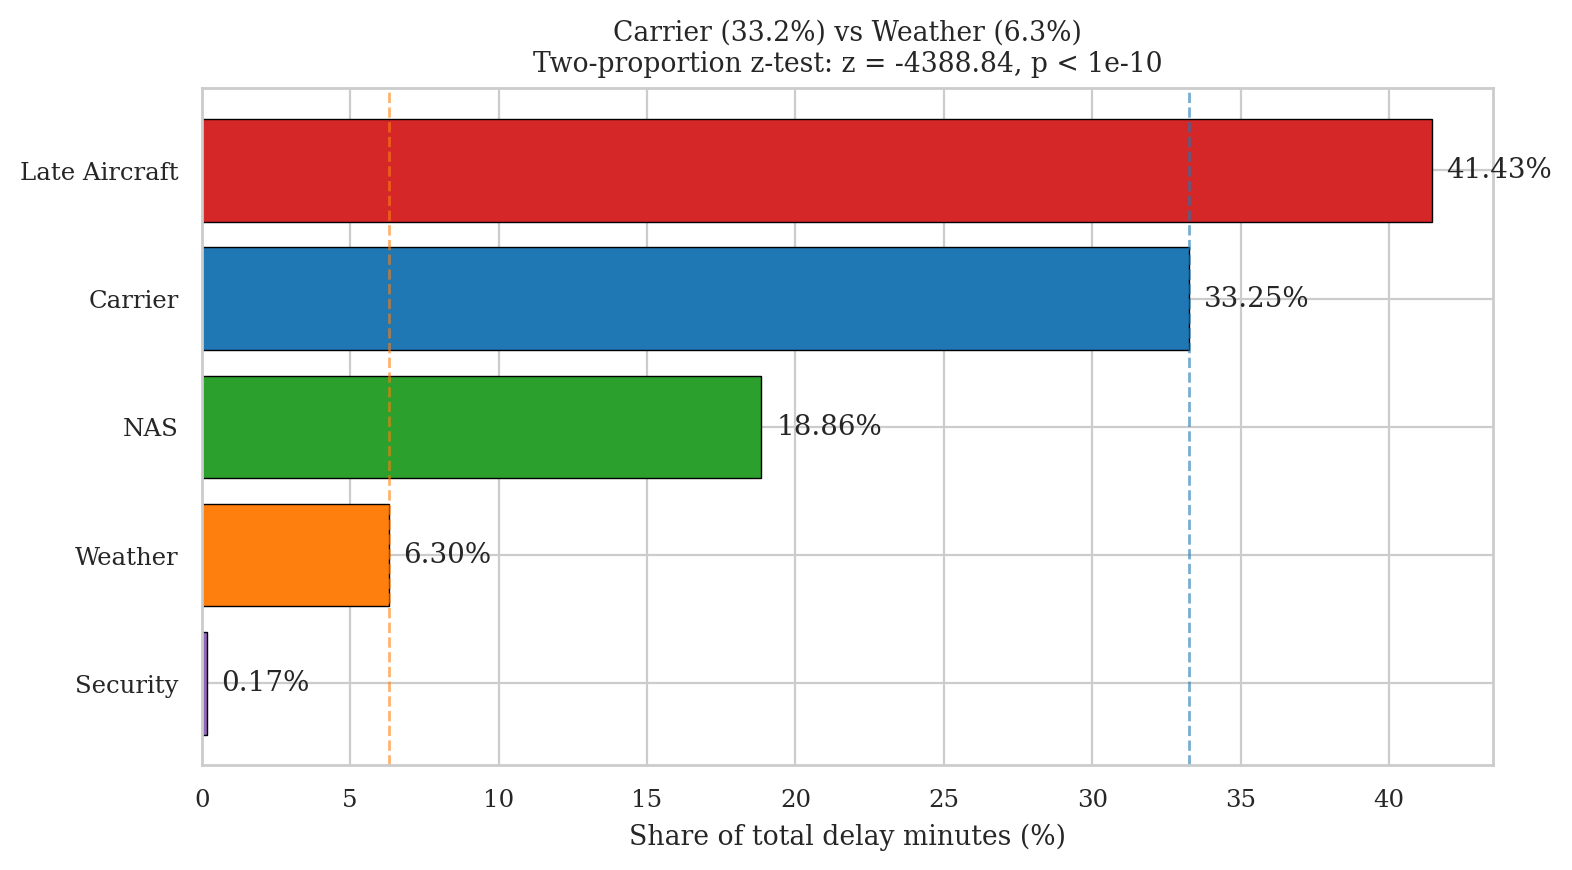
\includegraphics[width=0.82\linewidth]{fig_h3_weather_vs_carrier}
  \caption{Share of total delay minutes by cause category. The dashed
  vertical lines mark the carrier (33.25\%) and weather (6.30\%) shares
  whose equality is the null hypothesis of H3.}
  \label{fig:h3}
\end{figure}

\textbf{Decision: reject $H_0$.} Carrier-controllable causes account for
roughly $5.3\times$ as many delay minutes as weather, a difference whose
enormous z-statistic and tight confidence interval reflect the dataset's
$5\!\times\!10^7$-minute scale. The substantive implication is that
\emph{the leading drivers of delay are operational and propagation
factors, not weather}.

\subsection{H4: Flight Volume and Delay Rate}
\textbf{Test.} Pearson and Spearman correlation between airport-level
\texttt{total\_flights} (Jan--Aug 2024) and \texttt{delay\_rate}, plus
an OLS regression on $\log_{10}$ volume. We restrict to the 350 airports
with at least 100 flights to remove unreliable rates from very small
airports.

\textbf{Test statistics.} Pearson on raw volume: $r = 0.187$,
$p = 4.5\!\times\!10^{-4}$. Pearson on $\log_{10}$ volume: $r = 0.399$,
$p < 10^{-10}$. Spearman rank: $\rho = 0.422$, $p < 10^{-10}$. The
improvement from $r=0.187$ to $r=0.399$ when we log-transform volume
confirms the visual nonlinearity in Figure~\ref{fig:volume}: the
relationship is strong on the log scale but compressed on the raw
scale. The OLS fit
$\widehat{\text{delay\_rate}} = 0.128 + 0.0226 \cdot \log_{10}(\text{volume})$
has $R^2 = 0.159$, slope $t = 8.12$, $p < 10^{-10}$. The slope of
$0.0226$ means a tenfold increase in flight volume is associated with a
2.3-percentage-point increase in delay rate. The quintile boxplot in
Figure~\ref{fig:h4}(b) shows the same pattern in a distribution-free
way: median delay rate climbs monotonically from 0.176 (Q1) to 0.232
(Q5).

\begin{figure}[!htbp]
  \centering
  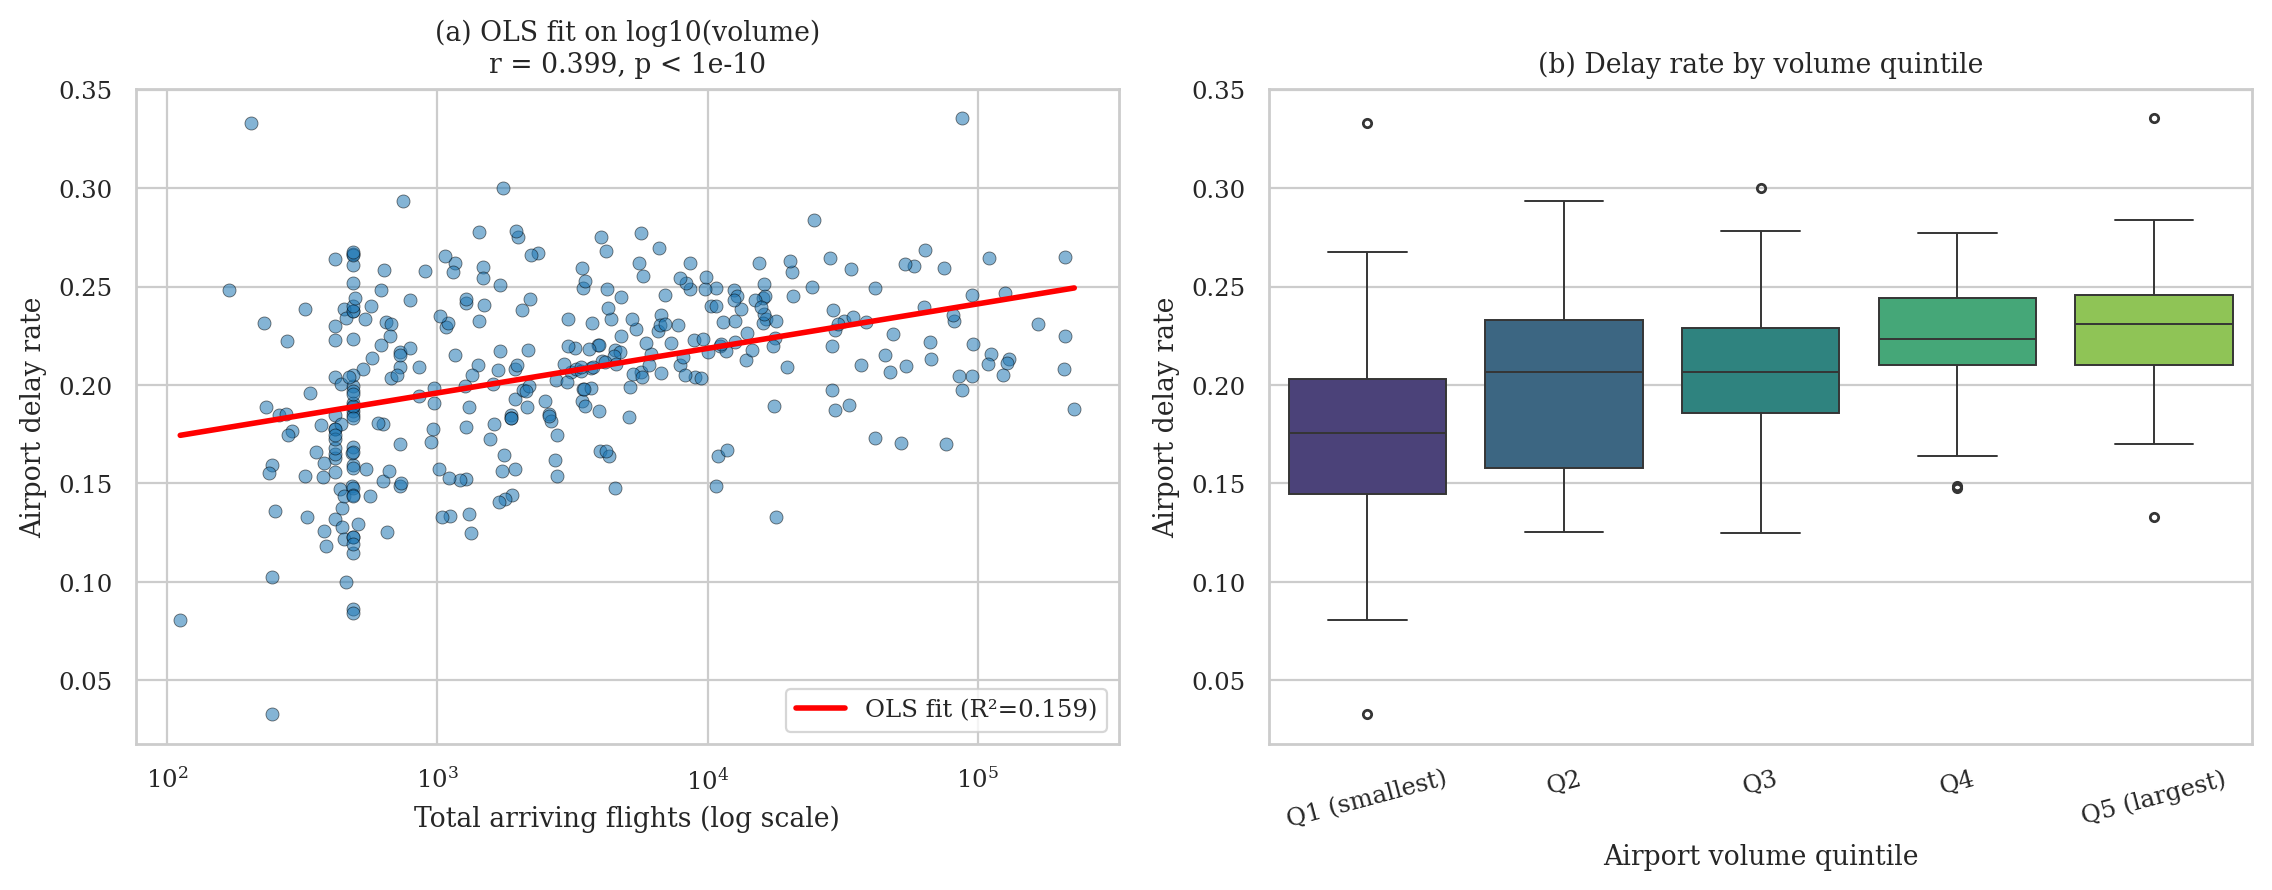
\includegraphics[width=\linewidth]{fig_h4_volume_regression}
  \caption{H4 visualization. (a) Each point is one of 350 airports; the
  red line is OLS on $\log_{10}$ volume. (b) Distribution of delay rate
  across volume quintiles; medians rise monotonically.}
  \label{fig:h4}
\end{figure}

\textbf{Decision: reject $H_0$.} There is a moderate, log-linear positive
relationship between airport volume and delay rate, but volume alone
explains only about 16\% of the variance in airport delay rates,
meaning carrier mix, geography, and weather climatology matter
substantially.

\subsection{Summary of Hypothesis Tests}
Table~\ref{tab:tests} consolidates the headline results.

\begin{table}[H]
\centering
\caption{Summary of inferential tests. All tests use $\alpha = 0.05$.}
\label{tab:tests}
\small
\renewcommand{\arraystretch}{1.10}
\begin{tabularx}{\linewidth}{l X r r l}
\toprule
\textbf{ID} & \textbf{Test} & \textbf{Statistic} & \textbf{p-value} & \textbf{Decision} \\
\midrule
H1 & ANOVA, carrier ($k\!=\!21$)            & $F=124.48$       & $<10^{-10}$ & Reject $H_0$ \\
H1 & Kruskal-Wallis, carrier                & $H=2{,}663.83$   & $<10^{-10}$ & Reject $H_0$ \\
H2 & ANOVA, month ($k\!=\!8$)               & $F=276.76$       & $<10^{-10}$ & Reject $H_0$ \\
H2 & Kruskal-Wallis, month                  & $H=2{,}174.47$   & $<10^{-10}$ & Reject $H_0$ \\
H3 & Two-proportion z, weather vs.\ carrier & $z=-4{,}388.84$  & $<10^{-10}$ & Reject $H_0$ \\
H4 & Pearson on $\log_{10}$ volume          & $r=0.399$        & $<10^{-10}$ & Reject $H_0$ \\
H4 & Spearman rank                          & $\rho=0.422$     & $<10^{-10}$ & Reject $H_0$ \\
\bottomrule
\end{tabularx}
\end{table}

\subsection{Multivariate Model Comparison}
The four univariate hypotheses give a yes/no verdict on each driver, but
they do not say how the drivers combine. To compare the relative
importance of carrier, season, volume, and cause-mix, we fit three
nested OLS regressions on the record-level data (each row is one
carrier-airport-month):
\begin{itemize}[leftmargin=2.0em, itemsep=1pt, topsep=1pt]
  \item \textbf{M1 (baseline):} \texttt{delay\_rate} $\sim$
  month dummies $+ \log_{10}(\texttt{arr\_flights})$. $p=8$ predictors.
  \item \textbf{M2 (+ carrier):} M1 plus 20 carrier dummies. $p=28$.
  \item \textbf{M3 (full):} M2 plus weather and NAS shares of total
  delay minutes per record. $p=30$.
\end{itemize}
We evaluate every model on three criteria: in-sample $R^2$, adjusted
$R^2$ to penalize model size, and 5-fold cross-validated $R^2$
(\texttt{sklearn}, shuffled, random state 42) to guard against
overfitting.

\begin{figure}[!htbp]
  \centering
  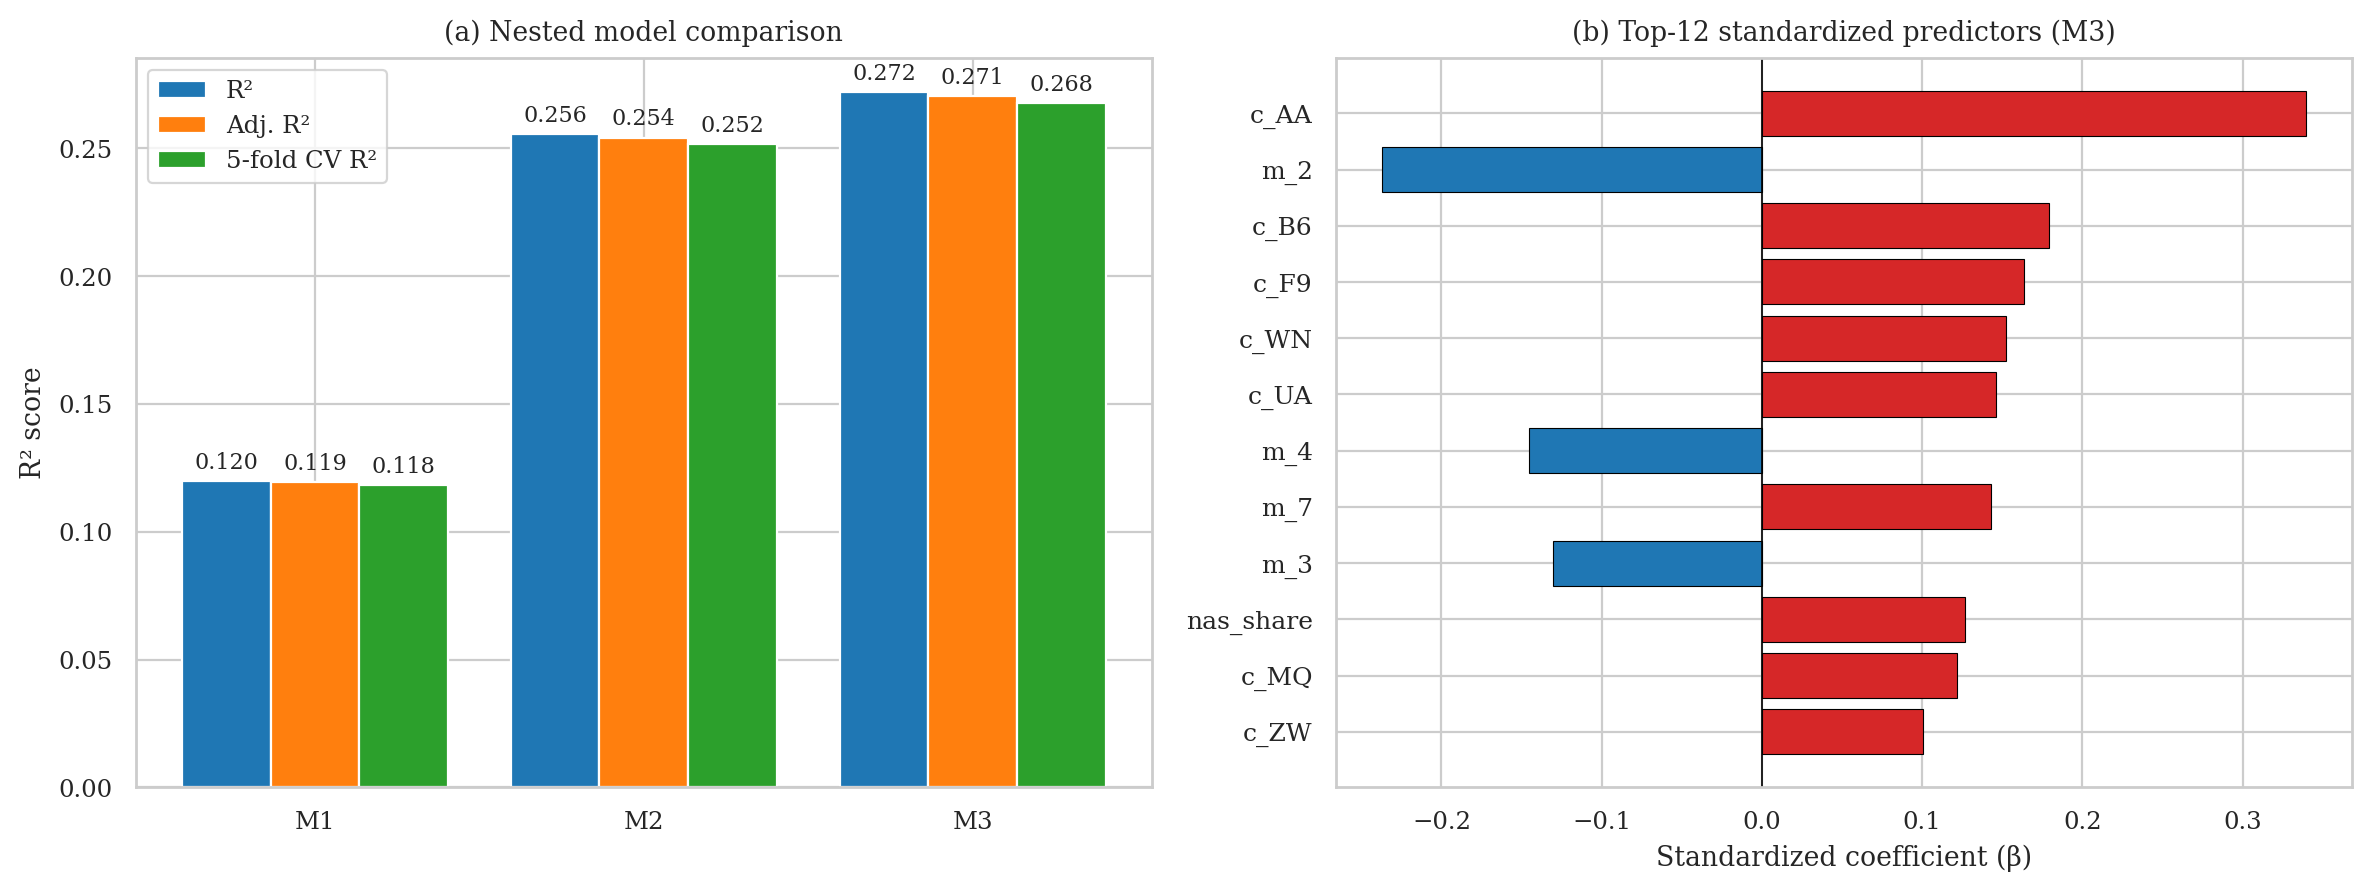
\includegraphics[width=\linewidth]{fig_model_comparison}
  \caption{Multivariate model comparison. (a) Three nested models
  evaluated on $R^2$, adjusted $R^2$, and 5-fold cross-validated $R^2$.
  Adding carrier identity (M1$\!\to\!$M2) more than doubles the
  explained variance; adding cause shares (M2$\!\to\!$M3) yields a
  smaller marginal improvement. (b) Top-12 standardized coefficients
  from M3; carrier AA dominates with $\beta=+0.34$.}
  \label{fig:models}
\end{figure}

The conclusion is unambiguous. M1 explains 12.0\% of variance; M2 lifts
$R^2$ to 25.6\%; the full model M3 reaches 27.2\%. Cross-validated $R^2$
tracks in-sample $R^2$ very closely (M3: $0.268 \pm 0.014$), giving us
confidence the gains are not artefacts of overfitting. The single
largest standardized coefficient in M3 is the AA carrier dummy
($\beta=+0.340$, i.e.\ AA is associated with a delay rate roughly
one-third of a standard deviation above the within-month/within-volume
baseline), followed by the February dummy ($\beta=-0.237$). Of the
top-12 standardized predictors, eight are carrier dummies and
four are month dummies. After controlling for volume,
carrier identity and seasonality dominate the explainable structure of
record-level delay rates.

% ===================== SECTION 4 =====================
\section{Geographic and Regional Extension}
\label{sec:geographic}

We enrich the analysis by joining the BTS data with a curated lookup of
latitude, longitude, U.S.\ state, and U.S.\ Census region for the 131
highest-traffic airports, which together account for 93.0\% of all
flights in the dataset.

\subsection{State-Level Tile-Grid Choropleth}
A geographically-positioned tile-grid representation of the U.S.\ lets us
read the regional structure at a glance without the visual distortions
introduced by Alaska, Hawaii, and the Mercator projection. Each state is
a single labeled cell carrying the mean delay rate (left panel of
Figure~\ref{fig:tilegrid}) and the share of delay minutes attributable
to weather (right panel).

\begin{figure}[!htbp]
  \centering
  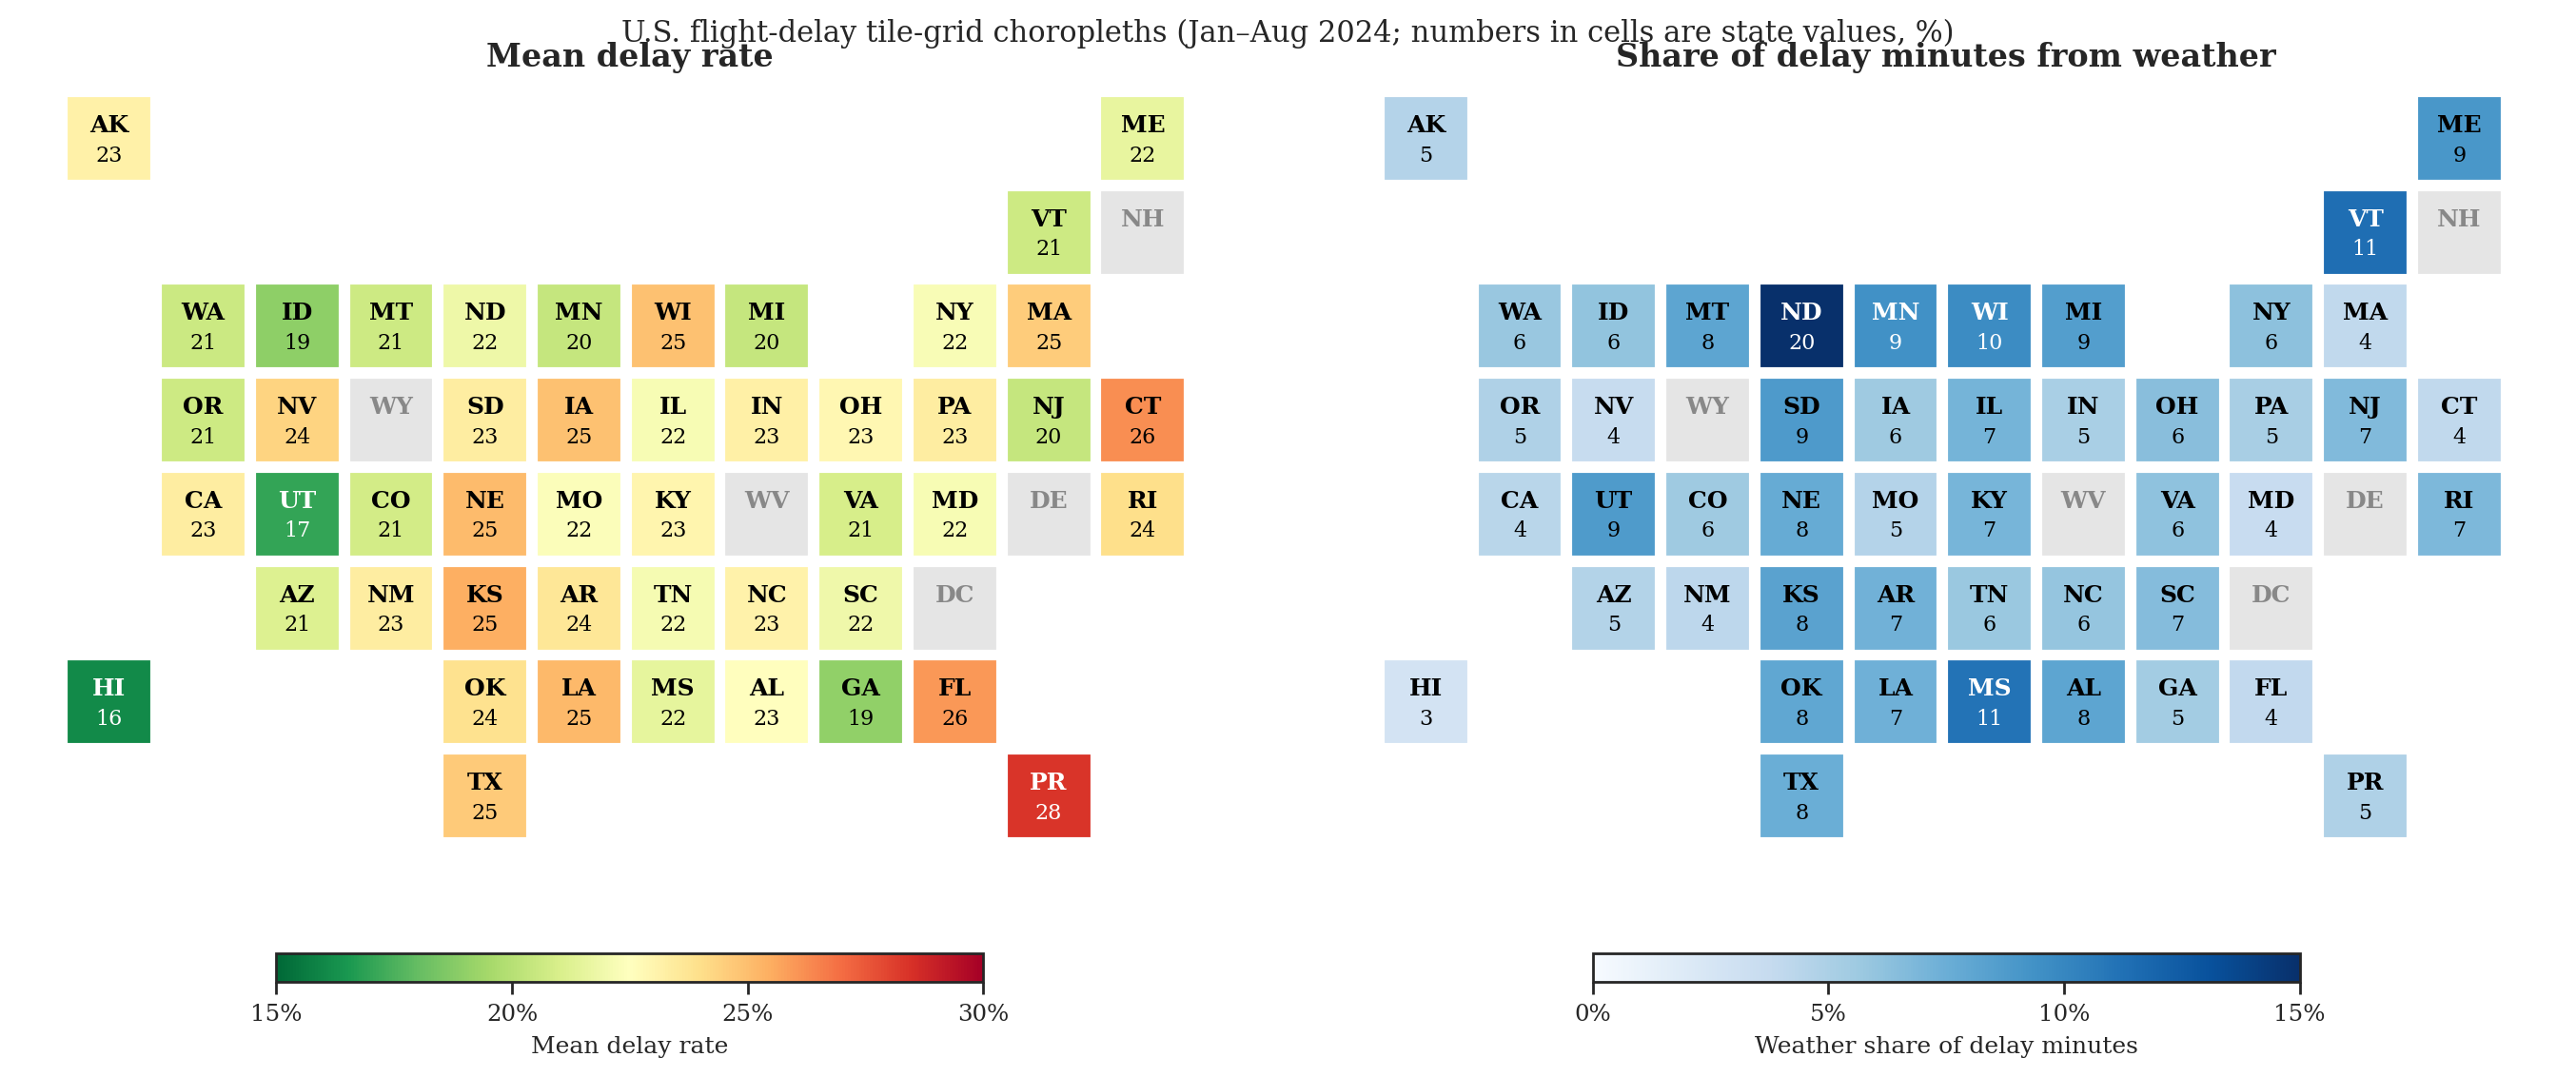
\includegraphics[width=\linewidth]{fig_us_tilegrid}
  \caption{State-level tile-grid choropleths for the 47 states with
  reporting airports. Numbers in cells are the state's value as a
  percentage. Left: mean delay rate. Right: weather's share of total
  delay minutes.}
  \label{fig:tilegrid}
\end{figure}

The two panels tell complementary stories. Mean delay rate (left) is
elevated across a southern arc from California's coastal hubs (LAS at
24\%, the Bay Area cluster around 23\%) through Texas, Louisiana,
Arkansas and Florida (FL = 26\%, second only to Puerto Rico at 28\%),
and up the Eastern Seaboard (CT = 26\%, NJ = 20\%, MA = 25\%). The
calmer states cluster in the upper Midwest and the Pacific Northwest,
with Hawaii at the floor (16\%) and Utah next (17\%). Weather share
(right) shows almost the inverse pattern: the upper Midwest (ND = 20\%,
MS = 11\%, MT = 8\%) and northern New England (VT = 11\%, ME = 9\%)
carry the highest weather burden, while the Sun Belt (FL = 4\%,
CA = 4\%, NV = 4\%) sees almost none. The two patterns together imply
that the South's high delay rates are driven by operational and
volume-related factors rather than meteorology.

\subsection{Bubble Map on the U.S. Land Outline}
Figure~\ref{fig:usmap} overlays the top-60 contiguous-U.S.\ airports on
a hand-traced outline of the country, with bubble size encoding traffic
volume and color encoding delay rate. The smaller gray dots represent
the remaining 290+ airports for spatial coverage.

\begin{figure}[!htbp]
  \centering
  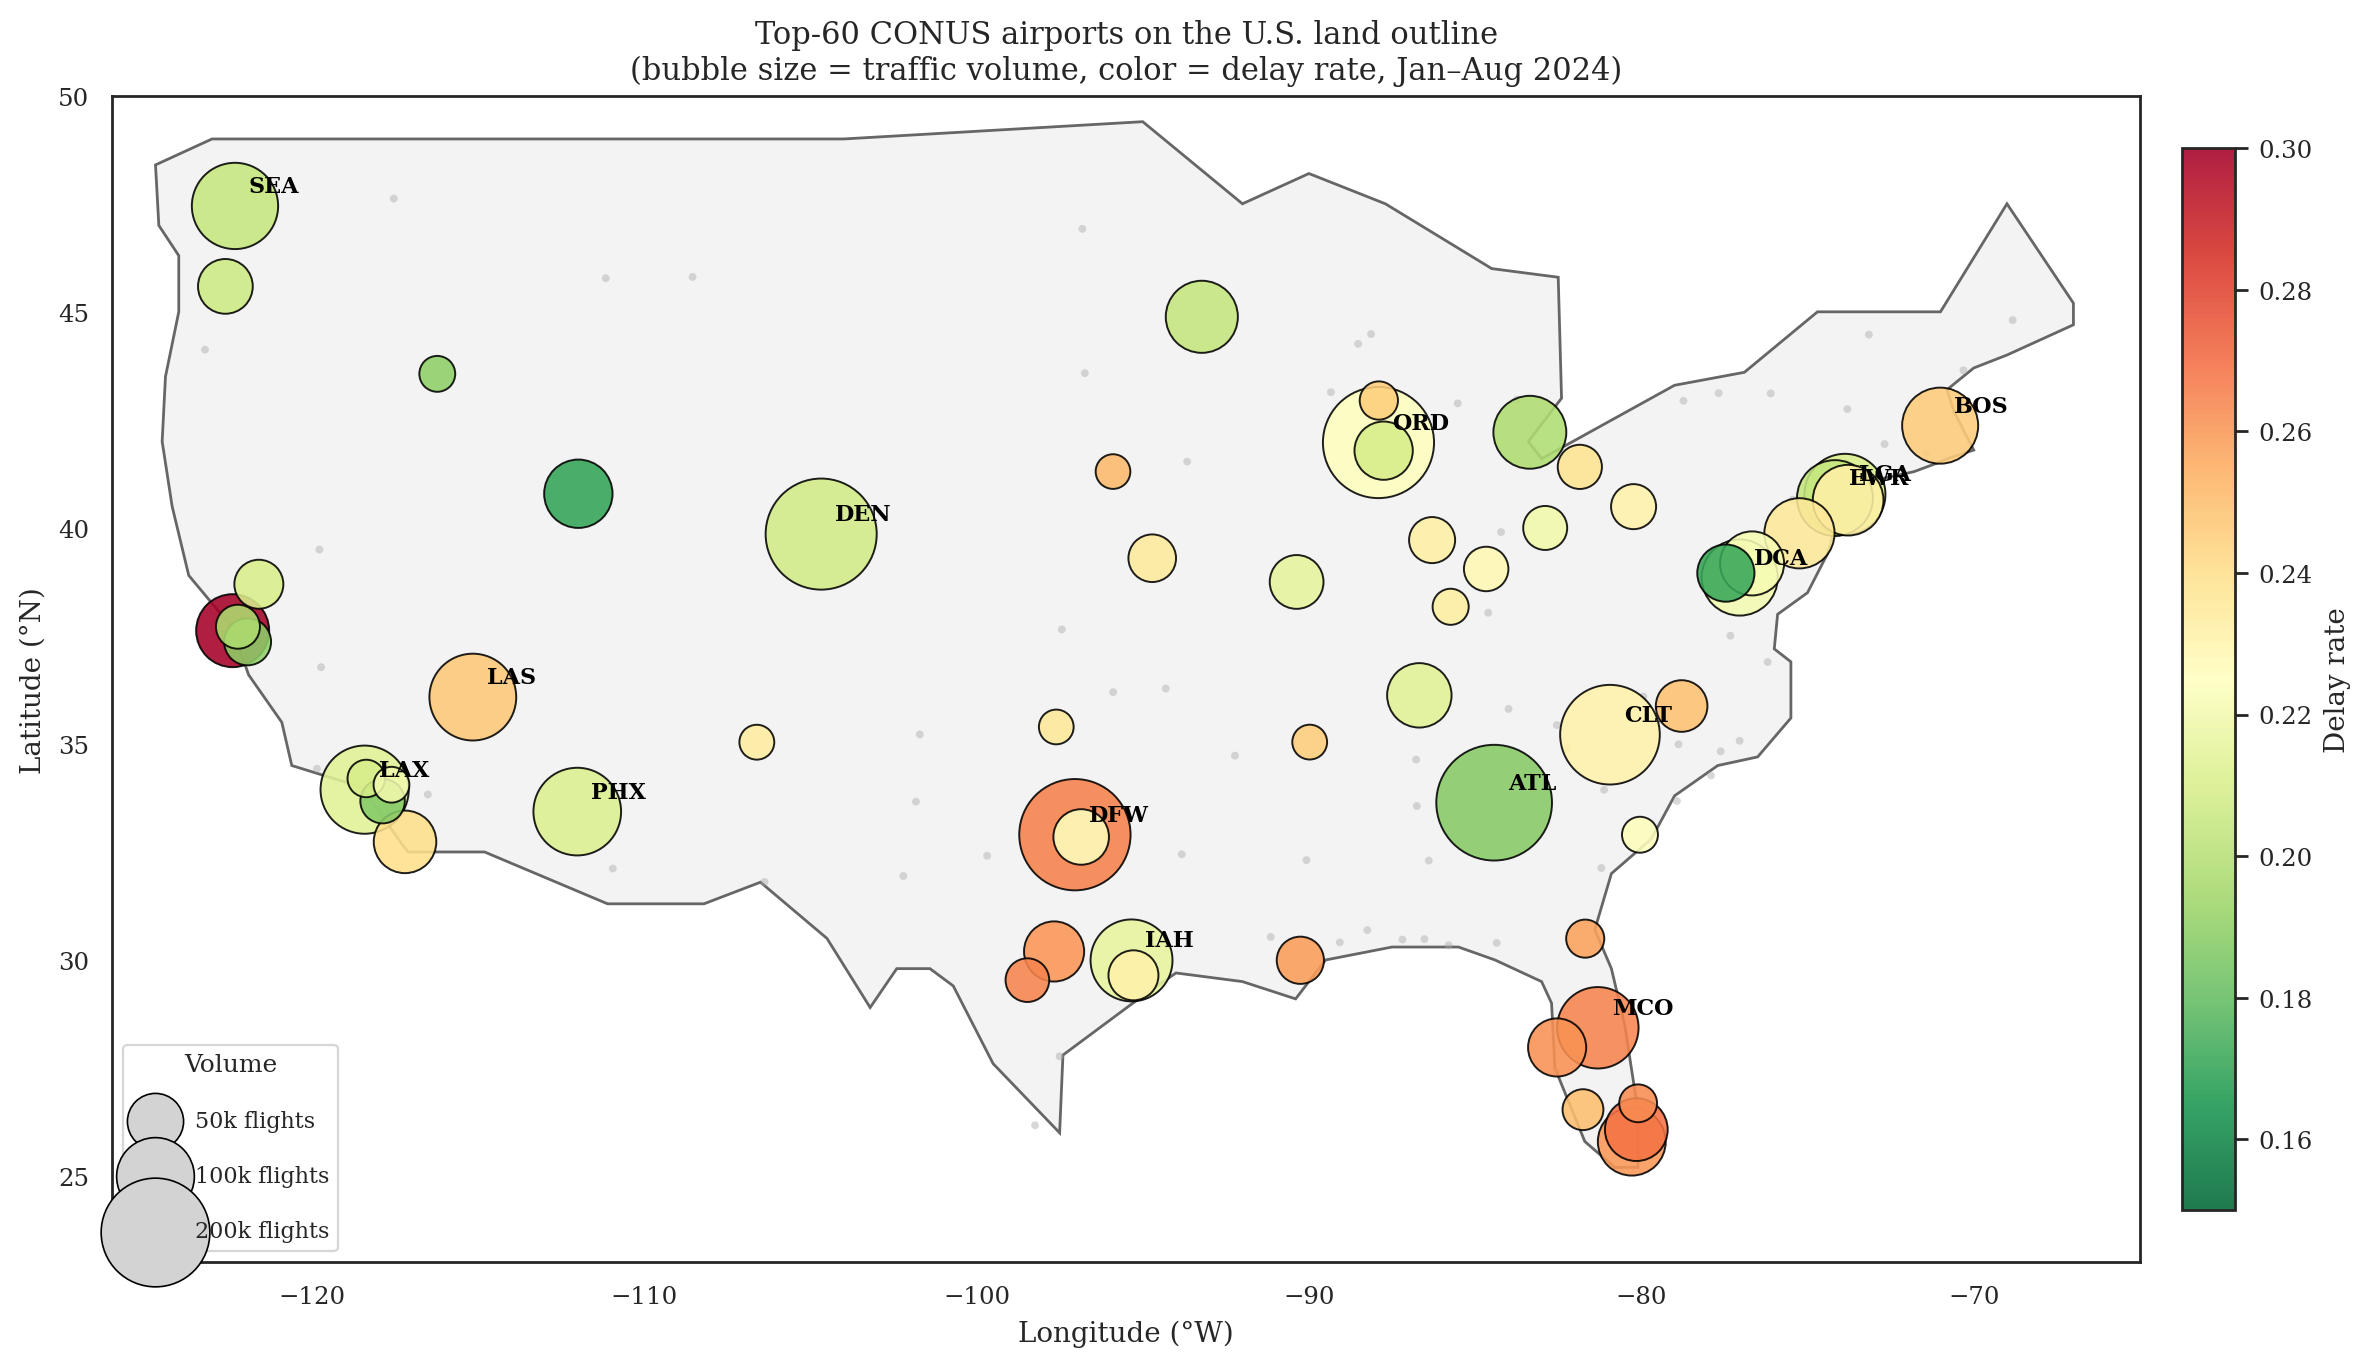
\includegraphics[width=\linewidth]{fig_us_outline_bubbles}
  \caption{Top-60 CONUS airports overlaid on a simplified U.S.\ land
  outline. Bubble size indicates total arriving flights (Jan--Aug 2024);
  color indicates the airport's delay rate. The gray background dots
  show all other reporting airports.}
  \label{fig:usmap}
\end{figure}

Three patterns are immediately legible from this view. The Texas-Florida
corridor shows the highest concentration of red bubbles (DFW, IAH, MCO,
and the smaller Florida airports), pointing to operationally challenging
conditions throughout the southern U.S.\ in the summer months that
dominate our panel. The Pacific Northwest, the Bay Area, and the Atlanta
hub appear in shades of green despite their large traffic volumes,
indicating that high volume on its own does not produce delays when
coupled with mature hub operations. Finally, the Northeast corridor
between Washington, DCA and Boston BOS shows a mixed pattern: heavy
volume but consistently high delay rates around the New York TRACON
(EWR, LGA, JFK), while DCA itself is the cleanest large airport in the
country at a delay rate near 0.16.

\subsection{U.S.\ Census Region Comparison}
Aggregating to the four U.S.\ Census regions (Northeast, Midwest,
South, West), a one-way ANOVA on airport-level delay rates yields
$F(3, 127) = 4.74$, $p = 3.6\!\times\!10^{-3}$; Kruskal-Wallis gives
$H = 20.67$, $p = 1.2\!\times\!10^{-4}$. We therefore reject the
hypothesis of regional homogeneity. Western airports have a median
delay rate of 0.209, well below the Midwest median of 0.234.
Interestingly, the cause-mix composition (Figure~\ref{fig:regional}b)
is much more uniform: weather is slightly more prominent in the
Northeast (5.7\%) than in the West (4.6\%), but Late Aircraft and
Carrier together dominate every region.

\begin{figure}[!htbp]
  \centering
  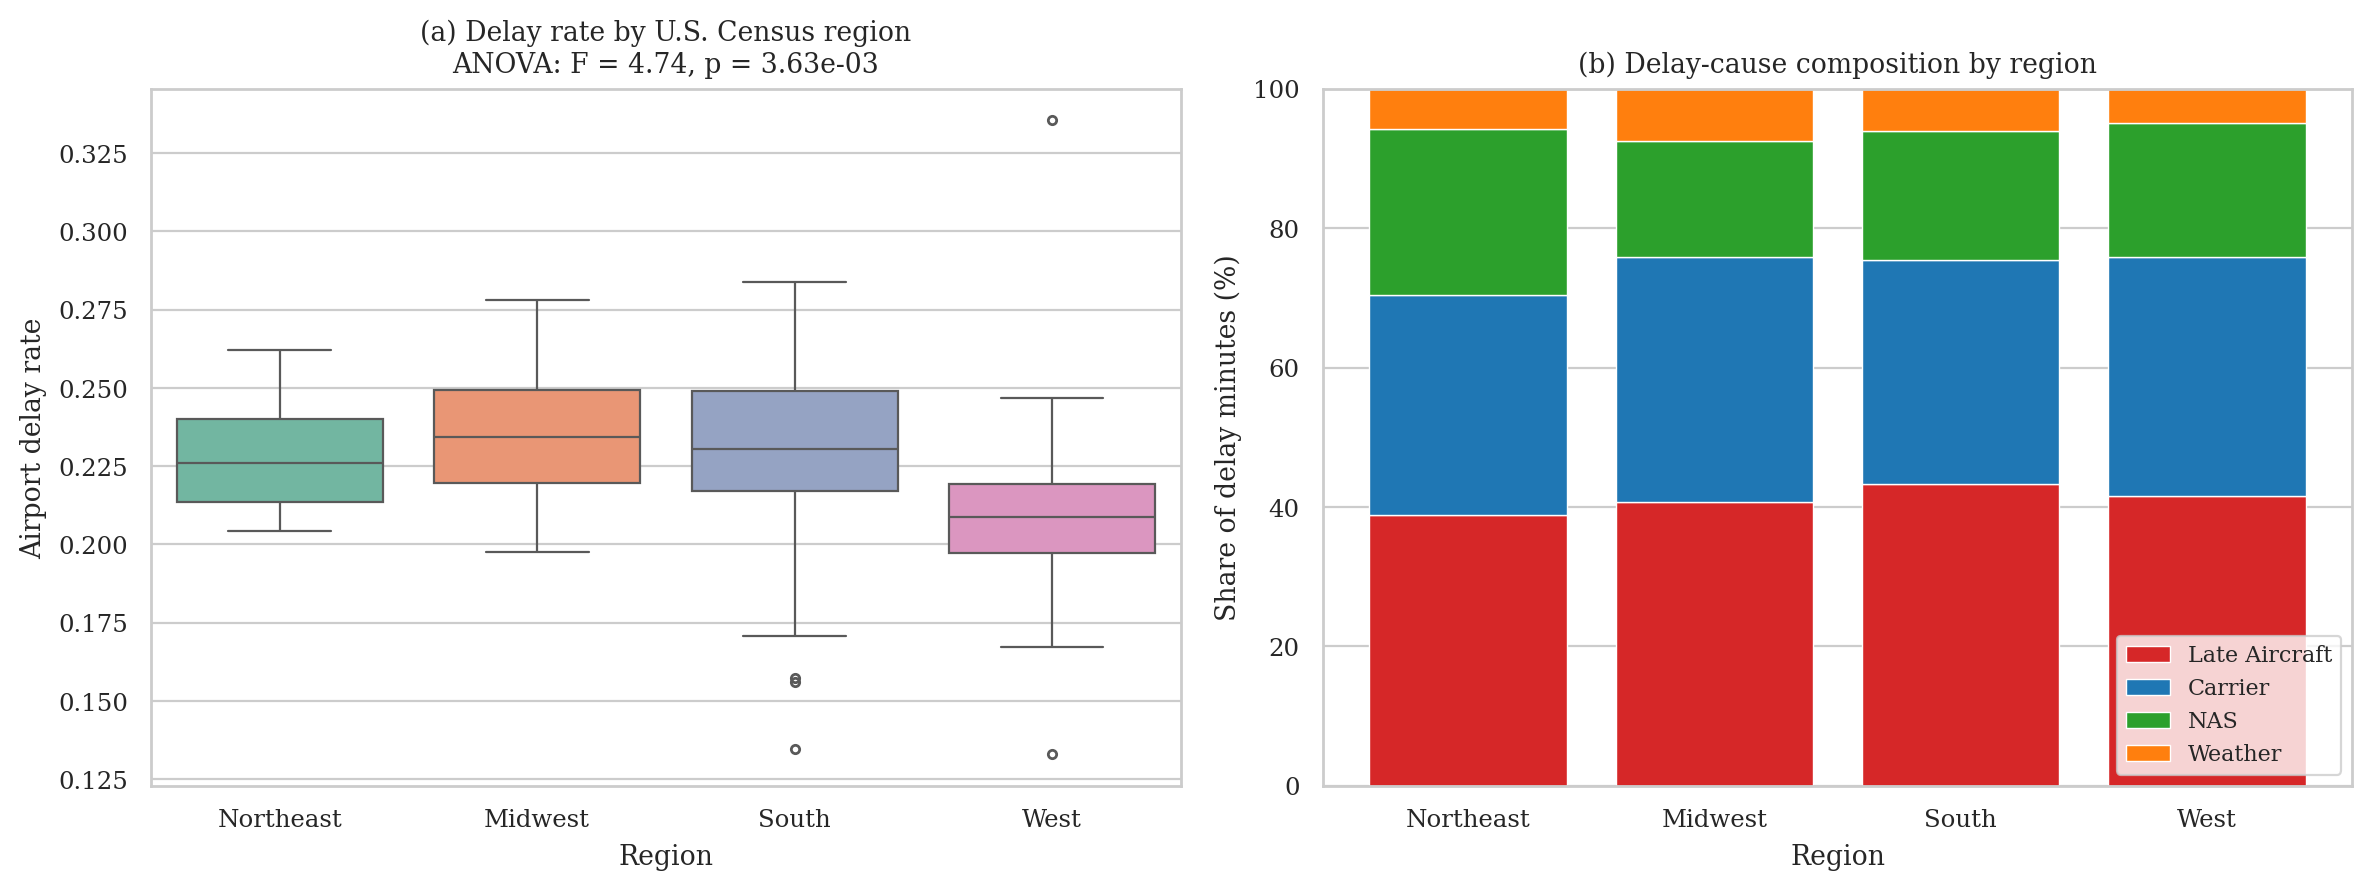
\includegraphics[width=\linewidth]{fig_regional}
  \caption{(a) Boxplot of airport delay rate by U.S.\ Census region.
  (b) Composition of total delay minutes by region; the regions are
  remarkably similar in cause mix.}
  \label{fig:regional}
\end{figure}

% ===================== SECTION 5 =====================
\section{Discussion and Conclusions}

\subsection{Summary of Findings}
Across the four pre-registered hypotheses we found overwhelming
evidence (every $p<10^{-10}$) that:
\textbf{(1) Carrier matters.} Mean delay rate differs across the 21
reporting carriers, with a more than two-fold range from PT
($\approx 0.13$) to AA ($\approx 0.30$) and a large effect size
$\eta^2 = 0.142$.
\textbf{(2) Season matters.} Delay rate varies significantly across the
eight months, with February the calmest and July the busiest; Tukey HSD
identifies a low-delay early-spring band and a high-delay summer band.
\textbf{(3) Carrier-controllable causes dwarf weather.} Carrier delay
accounts for 33.3\% of total delay minutes, while extreme weather
accounts for only 6.3\%, a $5.3\!\times$ ratio. Late-arriving
aircraft, which is itself almost entirely a carrier-network propagation
phenomenon, accounts for an additional 41.4\%.
\textbf{(4) Larger airports are slower.} A tenfold increase in flight
volume is associated with a 2.3-percentage-point increase in delay
rate, a moderate but highly significant log-linear relationship.

The multivariate model comparison shows that carrier identity is the
single most important predictor in our setting: adding it to a base
model of seasonality and volume more than doubles $R^2$
($0.120 \!\to\! 0.256$). This reinforces the policy implication that
meaningful reductions in U.S.\ domestic delay rates would require
addressing carrier-side operations rather than infrastructure or
weather alone.

\subsection{Operational and Policy Implications}
The dominance of carrier-controllable and late-arriving-aircraft
causes (74.7\% of all delay minutes combined) reframes the public
debate about flight delays. The intuitive narrative blames weather
and air-traffic-control bottlenecks, but the data show that these
factors together (NAS at 18.9\% plus weather at 6.3\%) explain only a
quarter of total delay minutes. The remaining three quarters are
operational decisions inside individual carriers: how aggressively
to schedule turnaround times, how much slack to build into crew
rosters, how quickly to recover from the first delayed leg of a
day. Three concrete policy implications follow.

First, performance-based incentives at the carrier level are likely
to deliver larger reductions in passenger delay-minute exposure than
incremental airport-infrastructure spending. The fact that two
similarly-sized carriers operating in the same airports can differ
by a factor of two in delay rate (PT versus AA in our panel)
demonstrates that the dominant variation is not environmental but
operational. Second, summer-season capacity planning should
explicitly model the carrier-specific buffer that determines whether
a thunderstorm produces a 30-minute or a 3-hour delay; our
carrier $\times$ month heatmap suggests that some carriers absorb
summer shocks while others amplify them. Third, the geographic
clustering of high-delay airports along the Texas-Florida corridor
points to a regional capacity-planning problem rather than a
nationwide one. The Pacific Northwest and the Atlanta hub demonstrate
that operational excellence is achievable; the Gulf Coast suggests
that the combination of summer convective weather, dense regional
networks, and tightly-scheduled hub banks creates a brittle system.

\subsection{Comparison with Prior Literature}
Our findings align with and extend several strands of the existing
flight-delay literature. \citet{kafle2017} estimate that
late-arriving aircraft propagation accounts for roughly one-third of
delays in any given period; we find 37.8\% of delayed flights and
41.4\% of delay minutes attributable to this cause, a slightly
higher share consistent with the post-pandemic recovery period from
which our 2024 data are drawn. \citet{rebollo2014} identify hub
centrality as a leading predictor in their network model; our H4
result that a tenfold increase in airport volume is associated with
a 2.3-percentage-point rise in delay rate is the cross-sectional
analogue of their network finding. \citet{abdelghany2004} report
clear monthly periodicities in arrival delays; our Tukey HSD analysis
of H2 confirms this with the additional structure that the eight
months partition into three statistically distinct regimes
(low-delay February-April, transition months, peak July).

The novel aspects of our contribution lie in the combination of
classical inference with a transparent nested-model comparison and a
geographic dimension. Most prior delay studies emphasize prediction
accuracy on flight-level data; we instead emphasize attribution at
the carrier-airport-month panel level, which is the unit at which
public policy operates. The carrier-versus-weather framing of H3, in
particular, is rarely tested directly in the literature even though
it sits at the heart of public discourse about delays.

\subsection{Limitations and Future Work}
Three limitations bound our conclusions. First, the panel covers only
January--August 2024; the high-volume November and December holidays
are missing, so we cannot speak to year-end seasonality. Second, the
DOT cause categories are reported by the carriers themselves: they can
sometimes classify ambiguous delays under NAS or weather rather than
under the carrier-controllable bucket, so our H3 finding is a
conservative estimate of the carrier share. Third, our analytical unit
is the carrier-airport-month, not the individual flight; we cannot
directly model propagation between specific flights, only the
aggregate footprint of late-arriving aircraft.

The most natural extensions of this work address each limitation in
turn. A flight-level study using the BTS T-100 database would
quantify how a delay at a hub airport cascades through the network.
Joining BTS to NOAA weather observations would let us control
explicitly for meteorology, providing a sharper upper bound on
weather's true contribution. A mixed-effects model with random slopes
by carrier would formally test the carrier-specific seasonality
patterns visible in the carrier $\times$ month heatmap. Finally,
extending the panel to a full calendar year would let us test whether
the post-pandemic recovery patterns observed here persist into the
high-volume holiday season.

\subsection{Innovativeness and Contribution}
Our contribution combines four classical inferential tests (ANOVA,
Kruskal-Wallis, two-proportion z, Pearson/Spearman) with a nested-model
comparison that quantifies driver importance, a state-level tile-grid
choropleth and bubble map that surface the regional clustering of
delay severity, and a Census-region ANOVA that complements the carrier
and seasonal analyses with a third axis of heterogeneity. The pipeline
is fully reproducible: all code, data, and figures sit in the
\textbf{project's GitHub repository} \citep{team8repo}, organized into four sequential scripts
(\texttt{01\_load\_and\_explore.py}, \texttt{02\_hypothesis\_tests.py},
\texttt{03\_geo\_and\_models.py}, \texttt{04\_us\_maps.py}) that re-run
end-to-end in well under a minute on a laptop.

\newpage

% ===================== REFERENCES =====================
\bibliographystyle{plainnat}
{\small
\setlength{\bibsep}{2pt}
\bibliography{references}
}

\end{document}
